% SIAM Article Template
\documentclass[r]{siamart171218}
% Packages and macros go here
\usepackage[english]{babel}
\usepackage{amsmath}
\usepackage{amssymb}
\usepackage{amsfonts}
\usepackage{array}
\usepackage{graphicx}
\usepackage{epsfig}
\usepackage{float}
%\usepackage{fullpage}
\usepackage{color}
\usepackage{enumitem}  
\usepackage{epstopdf}
\usepackage{stmaryrd}
\usepackage{standalone}
\usepackage{tikz, subfigure}
\usepackage{yfonts}

\usetikzlibrary{shapes, patterns, arrows}
\usetikzlibrary{calc}
\usepackage{pgfplots}
\usepgfplotslibrary{fillbetween}
\pgfplotsset{compat=1.16}

\usepackage{booktabs}  % for tables
\usepackage{capt-of}
\usepackage{multirow}
\usepackage[displaymath, mathlines]{lineno}


\newcommand{\fede}[1]{{\color{green}#1}}
\newcommand{\kent}[1]{{\color{red}#1}}
\newcommand{\miro}[1]{{\color{blue}#1}}
\newcommand{\paolo}[1]{{\color{magenta}#1}}
% Title. If the supplement option is on, then "Supplementary Material"
% is automatically inserted before the title.
%\title{On the weak coupling of 3D and 1D second order elliptic problems}
% \title{Coupling PDEs on 3D-1D domains\\ with Lagrange multipliers}
\title{Analysis and approximation of mixed-dimensional PDEs on 3D-1D domains coupled with Lagrange multipliers}

% Authors: full names plus addresses.
\author{M. Kuchta\thanks{Simula Research Laboratory, Oslo, Norway (\email{miroslav@simula.no})}\and F. Laurino\thanks{MOX, Department of Mathematics, Politecnico di Milano, Italy (\email{federica.laurino@polimi.it})} \and K.A. Mardal\footnotemark[1]$^{\;,}$\thanks{University of Oslo, Department of Mathematics (\email{kent-and@math.uio.no})} \and P. Zunino\thanks{MOX, Department of Mathematics, Politecnico di Milano, Italy (\email{paolo.zunino@polimi.it}), Corresponding Author}}

\begin{document}
\linenumbers

\maketitle

% REQUIRED
\begin{abstract}
Coupled partial differential equations defined on domains with different dimensionality are usually called mixed dimensional PDEs. We address mixed dimensional PDEs on three-dimensional (3D) and one-dimensional domains, giving rise to a 3D-1D coupled problem.
Such problem poses several challenges from the standpoint of existence of solutions and numerical approximation. For the coupling conditions across dimensions, we consider the combination of essential and natural conditions, basically the combination of Dirichlet and Neumann conditions. To ensure a meaningful formulation of such conditions, we use the Lagrange multiplier method, suitably adapted to the mixed dimensional case. The well posedness of the resulting saddle point problem is analyzed. Then, we address the numerical approximation of the problem in the framework of the finite element method. The discretization of the Lagrange multiplier space is the main challenge. Several options are proposed, analyzed and compared, with the purpose to determine a good balance between the mathematical properties of the discrete problem and flexibility of implementation of the numerical scheme. The results are supported by evidence based on numerical experiments.
\end{abstract}

% REQUIRED
\begin{keywords}
mixed dimensional PDEs, finite elemet approximation, essential coupling conditions, Lagrange multipliers
\end{keywords}

% REQUIRED
\begin{AMS}
n.a.
\end{AMS}

% >>>>>>>>>>>>>>>>>>>>>>>>>>>>>>>>>>>>>>>>>>>>>>>>>>>>>>>>>>>>>>>>>>>>>>>>>>>>>>>>>>>>>>>>>>>>>>>>>>>>
 
% definitions here

\def\ud{u_{\odot}}
\def\vd{v_{\odot}}
\def\ld{\lambda_{\odot}}
\def\udh{u_{\odot h}}
\def\udfh{u_{\odot \fkh}}
\def\vdh{v_{\odot h}}
\def\vdfh{v_{\odot \fkh}}
\def\ldh{\lambda_{\odot h}}
\def\md{\mu_{\odot}}
\def\mdh{\mu_{\odot h}}
\def\lld{l_{\odot}}
\def\uf{u_{\ominus}}
\def\up{u_{\oplus}}
\def\eps{\epsilon}
\def\nn{\boldsymbol n}
\def\rr{\boldsymbol r}
\def\RR{\boldsymbol R}
\def\kk{\boldsymbol k}
\def\ss{\boldsymbol s}
\def\uu{\boldsymbol u}
\def\vv{\boldsymbol v}
\def\xx{\boldsymbol x}
\def\bu{\overline{u}}
\def\bv{\overline{v}}
\def\tu{\widetilde{u}}
\def\tv{\widetilde{v}}
\def\TT{\boldsymbol T}
\def\NN{\boldsymbol N}
\def\BB{\boldsymbol B}
\def\ttu{\widetilde{\widetilde{u}}}
\def\ttv{\widetilde{\widetilde{v}}}
\def\cv{\check{v}}
\def\mesh{{\cal T}^h}
\def\ball{{\cal B}}
\def\R{\mathbb{R}}
\def\D{\mathcal{D}}
\def\DD{\partial\mathcal{D}}
\def\trace{{\mathcal{T}_\Gamma}}
\def\mtrace{{\overline{\mathcal{T}}_\Lambda}}
\def\ext{\mathcal{E}_\Gamma}
\def\ide{\mathcal{I}}
\def\ii{\hat{\imath}}
\def\fkh{\mathfrak{h}}
\newcommand{\avrd}[1]{\overline{\overline{#1}}}
\newcommand{\avrc}[1]{\overline{#1}}
\newcommand{\refe}[1]{{#1}_{\mathrm{ref}}}
\newcommand{\norm}[1]{\lVert{#1}\rVert}

\newcommand{\vertiii}[1]{{\left\vert\kern-0.25ex\left\vert\kern-0.25ex\left\vert #1 
    \right\vert\kern-0.25ex\right\vert\kern-0.25ex\right\vert}}

\newtheorem{thm}{Theorem}[section]
\newtheorem{prop}{Property}[section]
\theoremstyle{remark}
\newtheorem{remark}{Remark}[section]
 
% >>>>>>>>>>>>>>>>>>>>>>>>>>>>>>>>>>>>>>>>>>>>>>>>>>>>>>>>>>>>>>>>>>>>>>>>>>>>>>>>>>>>>>>>>>>>>>>>>>>>
\section{Introduction}\label{sec:intro}

In this study we consider coupled partial differential equations on domains with mixed dimensionality, in particular we address the  3D-1D case. The mathematical structure of such problems can be represented by the following formal equations:
\begin{subequations}
\label{eq:pde}
\begin{align}
\label{eq:pde1}
  -\Delta u + u + \lambda \delta_{\Lambda} &= f &\mbox{ in } \Omega,\\
\label{eq:pde2}
 d_s^2 \ud + \ud - \lambda &= g &\mbox{ on } \Lambda,\\
\label{eq:coupling}
\mathcal{T}_\Lambda u - \ud  &=  \paolo{q} &\mbox{ on } \Lambda . 
\end{align}
\end{subequations}
Problem \eqref{eq:pde} can be described as an example of \emph{mixed dimensional PDEs}.
Here, $u$, $\ud$,  $\lambda$ are unknowns,  $\Omega$ is a bounded domain in $\R^3$, whereas $\Lambda \subset \Omega$ is a 1D structure
parameterized in terms of $s$ and $d_s$ is the derivative with respect to $s$. 
The term $\lambda\delta_{\Lambda}$ is a Dirac measure such that 
$\int_{\Omega}\lambda(x)\delta_{\Lambda}v(x)\,\mathrm{d}x=\int_{\Lambda}\lambda(t)v(t) \,\mathrm{d}t$
for a continuous function $v$ and $\mathcal{T}_\Lambda: \Omega\rightarrow\Lambda$ is a suitable restriction operator from 3D to 1D. 

Using models based on mixed dimensional PDEs is motivated by the fact that many problems in geo- and biophysics are characterized by slender cylindrical structures coupled to a larger 3D body, where the characteristic transverse length scale of the slender structure is many orders of magnitude smaller than the longitudinal length.  For example, in geophysical applications the radii of wells are often of the order of 10 cm while the length may be several kilometers~\cite{Peaceman1978183, Peaceman1983531}. Similarly, in applications involving the blood flow and oxygen transport of the micro-circulation the capillary radius is a few microns, while simulations are often performed on mm to cm scale, with thousands of vessels~\cite{berg2020modelling,fang2008oxygen,gould2017capillary, secomb2004green}. Finally, in neuro-science applications a neuron has width of a few microns, while  its length is much longer. For example, an axon of a motor neurons may be as long as a meter.  Hence,  at least 4 orders of magnitude in difference in transverse and longitudinal direction is common in both geo-physics, bio-mechanics and neuro-science. Meshes dictated by resolving the transverse length scale in 3D would then possibly lead to the order of $10^{12}$ degrees of freedom. Even if adaptive and strongly anisotropic meshes are allowed for, the computations quickly become demanding if many slender structures and their interactions are under study.  

From a mathematical standpoint, the challenge involved in problem \eqref{eq:pde} is that neither $\mathcal{T}_\Lambda$ nor $\delta_\Lambda$ are well defined. That is, without extra regularity,  solutions of elliptic PDEs only have well defined traces of co-dimension one. Here, $\mathcal{T}_\Lambda$ is of co-dimension two, mapping functions defined on a domain in 3D to functions defined along a 1D curve. 
The challenge of coupling PDEs on domains with high dimensionality gap has recently attracted the attention of many researchers. The sequence of works by D'Angelo, \cite{DAngelo,d2012finite,d2008coupling} have remedied the well-posedness by weakening the solution concept. The approach naturally leads to non-symmetric formulations. An alternative approach is to decompose the solution into smooth and non-smooth components, where the non-smooth component may be represented in terms of Green's functions, and then consider the well-posedness of the smooth component \cite{gjerde2019singularity}. The numerical approximation of such equations has been also studied in a series of works. The consistent derivation of numerical approximation schemes for PDEs in mixed dimension is addressed in \cite{Nordbotten}. Concerning approximability,  elliptic equations with Dirac sources represent an effective prototype case that has been addressed in \cite{Bertoluzza201897,koppl2016local,koppl2014optimal}, where the optimal a-priori error estimates for the finite element approximation are derived. Furthermore, the interplay between the mathematical structure of the problem and solvers, as well as preconditioners for its discretization has been studied in details  in \cite{kuchta2016preconditioners} for the solution of 1D differential equations embedded in 2D, and more recently extended to the 3D-1D case in \cite{KMM2}.

Stemming from this literature, in this work we adopt and analyze a different approach, closely related to \cite{KVWZ,laurino_m2an}. That is, we exploit the fact that $\Lambda$ is not strictly a 1D curve, but rather a very thin 3D structure with a cross-sectional area far below from what can be resolved. With this additional assumption, we show that robustness with respect to the cross-sectional area can be restored. The major novelty with respect to the previous works is that we address essential type coupling conditions, namely Dirichlet-Neumann conditions, rather than natural type ones, such as the Neumann-Robin or Robin-Robin cases. These coupling conditions pose additional difficulties as the conditions 
are not a natural part of the weak formulation of the problem. We overcome this difficulty by  resorting to a weak formulation of the Dirichlet-Neumann coupling conditions across dimensions by using Lagrange multipliers.

\paolo{Although the focus of the present work is mostly about analysis and approximation of the proposed approach, we stress that it aims to build the mathematical foundations to tackle various applications involving 3D-1D mixed dimensional PDEs, such as FSI of slender bodies \cite{Mori2019887}, microcirculation and lymphatics \cite{Possenti2019101,Vinje2019}, subsurface flow models with wells \cite{Cerroni2019} and the electrical activity of neurons.}

%>>>>>>>>>>>>>>>>>>>>>>>>>>>>>>>>>>>>>>>>>>>>>>>>>
\section{Preliminaries}\label{sec:setting}

Let the domain $\Omega\subset \R^3 $ be convex and composed of two parts, 
$\Omega_{\ominus}$ and $\Omega_{\oplus}:=\Omega\setminus\overline{\Omega}_{\ominus}$. 
Let 
$\Omega_{\ominus}$ be a \emph{generalized cylinder}, c.f.  \cite{MR1940257}, 
that is; the swept volume of a two dimensional set, $\partial\mathcal{D}$, moved along a curve, $\Lambda$, in the three-dimensional domain, $\Omega$, see for Figure \ref{fig1} for an illustration. 
In detail, the curve 
$\Lambda = \{\boldsymbol \lambda(s), \ s\in(0,S)\}$,  where 
$\boldsymbol \lambda(s) = [\xi(s), \tau(s), \zeta(s)], \ s\in(0,S)$ is a $\mathcal{C}^2$-regular curve in the three-dimensional domain $\Omega$.
For simplicity, let us assume that $\|\boldsymbol \lambda^\prime(s)\|=1$ such that the arc-length and the coordinate $s$ coincide.
Further, let $\mathcal{D}(s) = [x(r,t),y(r,t)]: (0,R(s))\times(0,T(s)) \rightarrow \R^2$ be a parametrization of the cross section
and $\Gamma$ be the lateral surface of $\Omega_{\ominus}$, i.e.
$\Gamma=\{ \ \partial \mathcal{D}(s) \  | \ s \in \Gamma\}$,
while the upper and lower faces of $\Omega_{\ominus}$ belong to $\partial\Omega$. 
We assume that $\Omega_{\ominus}$ crosses $\Omega$ from side to side.
 \paolo{Finally, $|\cdot|$ denotes the Lebesgue measure of a set, e.g. $|\mathcal{D}(s)|$ is the cross-sectional area of the cylinder. In general, $|\D(s)|$ must be strictly positive and bounded.}
According to the geometrical setting, we will denote with $v,\,v_\oplus,\,v_\ominus,\,\vd$,
functions defined on $\Omega,\,\Omega_{\oplus},\,\Omega_{\ominus},\,\Lambda$, respectively.

Let $D$ be a generic regular bounded domain in $\R^3$ and $X$ be a Hilbert space defined on $D$. Then  $(\cdot,\cdot)_X$ and $\|\cdot\|_X$ denote the inner product and norm of $X$, respectively.
The duality pairing between the $X$ and its dual $X^*$ is denoted as $\langle\cdot,\cdot\rangle$.
Let $(\cdot,\cdot)_{L^2(D)}$,  $(\cdot,\cdot)_D$ or simply $(\cdot,\cdot)$ be the $L^2(D)$ inner product on $D$.
We use the standard notation $H^q(D)$ to denote the Sobolev space of functions on $D$ with all derivatives up to the order $q$ in $L^2(D)$.
The corresponding norm is $\|\cdot\|_{H^q(D)}$ and the seminorm is $\vert\cdot\vert_{H^q(D)}$.
The space $H^q_0(D)$ represents the closure in $H^q(D)$ of smooth functions with compact support in $D$.



Let $\Sigma$ be a Lipschitz co-dimension one subset of $D$. We denote with $\mathcal{T}_\Sigma: H^q(D) \rightarrow H^{q-\frac 1 2}(\Sigma)$ the trace operator from \kent{$D$} to $\Sigma$.
The space of functions in $H^{\frac 1 2}(\Sigma)$ with continuous extension by zero outside $\Sigma$ is denoted 
$H^{\frac 1 2}_{00}(\Sigma)$ and we remark that 
$H^{\frac 1 2}_{00}(\Sigma) = \mathcal{T}_\Sigma H^1_0(D)$
and  $H^{-\frac 1 2}(\Sigma) = (H^{\frac 1 2}_{00}(\Sigma))^*$

\begin{figure}[t!]
\begin{center}
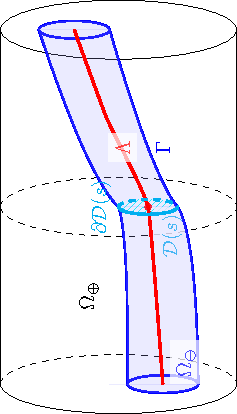
\includegraphics[width=0.35\textwidth,angle=-90]{./graphics/domain.tex}
\end{center}
\caption{Geometrical setting of the problem}
\label{fig1}
\end{figure}


\kent{
We will frequently use inner products and norms that are weighted. The
$L_2$ and $H^1$ inner products
weighted by a scalar function 
$w$, which is strictly positive and bounded almost everywhere,
are defined as 
follows
\begin{equation*}
%(u,v)_{\Gamma, w} = 
(u,v)_{L^2(\Omega), w} = 
\int_{\Omega} w \, u \, v d\omega \ \mbox{   and   } \
%(u,v)_{\Gamma, w} = 
(u,v)_{H^1(\Omega), w} = 
\int_{\Omega}  w \, u \, v d\omega
+ \int_{\Omega} w \, \nabla u \cdot \nabla v d\omega
\end{equation*}
whereas a weighted fractional
space \miro{$H^s(\Gamma; w)$} is defined in terms of the interpolation of the corresponding weighted spaces. 
For the norm of such spaces, we introduce 
the Riesz map $S$ such that 
for $u, v \in H^1(\Gamma)$ we have 
\[
(S u,v)_{H^1(\Gamma),w} = (u,v)_{L^2(\Gamma), w}.
\]
Then $S$ is a compact self-adjoint operator. 
Assuming that $\{\lambda_k\}_k$ is the set of eigenvalues, 
$\{\phi_k\}_k$ the set of eigenvectors of $S$ 
orthonormal with respect to the inner 
product $(\cdot, \cdot)_{L^2(\Gamma), w}$ and $u\in H^1(\Gamma)$ can be expressed 
as $u=\sum_k c_k \phi_k$ 
then
\[
\|u\|^2_{H^s(\Gamma), w} = \sum_k \lambda_k^{-s} c_k^2 .   
\]
The space $H_{00}^s(\Gamma; w)$ is defined analogously, but with $S$ above defined in terms of the $H^1_0$ inner product. Owing to the positivity and boundedness of $w$ the weighted spaces equal the corresponding non-weighted spaces as sets, but their norms are different.
 }

Central in our analysis are the transverse averages $\avrc{w},\,\avrd{w}$ defined as, 
\begin{gather*}
\avrc{w}(s) = |\partial\mathcal{D}(s)|^{-1} \int_{\partial\mathcal{D}(s)} w d\gamma \quad \mbox{and} \quad 
\avrd{w}(s) = |\mathcal{D}(s)|^{-1} \int_{\mathcal{D}(s)} w d\sigma, 
\end{gather*}
where $d\omega, \ d\sigma, \ d\gamma$ are the generic volume, surface and curvilinear Lebesgue measures.
Clearly, 
\begin{gather*}
\int_{\Omega_{\ominus}} w d\omega 
= \int_\Lambda \int_{\mathcal{D}(s)} w d\sigma ds
= \int_\Lambda |\mathcal{D}(s)|\avrd{w}(s) ds\, 
\\
\int_{\partial\Omega_{\ominus}} w d\sigma 
= \int_\Lambda \int_{\partial\mathcal{D}(s)} w d\gamma ds
= \int_\Lambda  |\partial \mathcal{D}(s)| \avrc{w}(s) ds\,. 
\end{gather*}
Analogously, for functions defined on $\Lambda$ and $\Omega_\ominus$ respectively, 
we let  $d_s$ and $\partial_s$ be the ordinary and partial derivative with respect to the arclength.

The operator obtained from a combination of the average operator $\avrc{(\cdot)}$ with the trace on $\Gamma$ will be denoted with $\mtrace = \avrc{(\cdot)} \circ \trace$, as it maps functions on $\Omega$ to functions on $\Lambda$.
Further, let the extension operator $\mathcal{E}_{\Gamma}: H^{\frac 1 2}_{00}(\Lambda) \rightarrow H^{\frac 1 2}_{00}(\Gamma)$ be defined such that $(\mathcal{E}_{\miro{\Gamma}}\vd)(x)=\vd(s)$, for any $x\in \DD(s)$. Then, the following identity shows that the transversal uniform extension operator is the inverse of the transversal average,
\begin{equation}\label{eq:ext}
\langle \mtrace u, \vd \rangle_{\Lambda, |\DD|} 
= \int _{\Lambda} |\DD| \left( \frac{1}{|\DD|} \int_{\DD} \trace u \, d\gamma \right) \vd \, ds 
= \langle \trace u, \ext \vd\rangle_{\Gamma}\,.
\end{equation}

%From the theory of interpolation of Sobolev spaces we define the fractional norms $\|\cdot \|_{H^{\frac 12}_{00}(\Gamma)}$ and $\|\cdot \|_{H^{\frac 12}_{00}(\Lambda)}$ as functions of the eigenvalues and eigenfunctions of the Laplacian on $\Gamma$ and $\Lambda$ respectively, see for example \cite{MR0350177,MR2328004}. 
%We denote as $\phi _{ij}$ and $\rho _{ij}$, for $i=1,2,\dots$, $j=0,1,\dots$, the eigenfunctions and the eigenvalues of the Laplacian on $\Gamma$ with homogeneous Dirichlet condition at the boundary. Then, the norms of $H^{\frac 12}_{00}(\Gamma),\,H^{\frac 12}_{00}(\Lambda)$ and the corresponding dual norms are defined as
%\begin{equation}\label{eq:fracnorm_gamma}
%\|u\|_{H^{\frac 12}_{00}(\Gamma)}=\left(\sum_{i=1}^{\infty}\sum_{j=0}^{\infty} \left( 1+ \rho_{ij}\right)^{\frac 12}|a_{ij}|^2\right)^{\frac 12}
%\ \text{with} \ a_{ij}=\left( u,\phi _{ij} \right)_{\Gamma};
%\quad
%\| v \|_{H^{-\frac 12}(\Gamma)} = \sup_{u\in H^{\frac 12}_{00}(\Gamma)}\frac{\langle u, v \rangle_\Gamma}{\|u\|_{H^{\frac 12}_{00}(\Gamma)}}\,.
%\end{equation}

%We define the equivalent weighted norm in $H^{\frac 12}_{00}(\Lambda)$ in the same way,
%\begin{equation}\label{eq:weightfracnorm}
%\|u\|_{H^{\frac 12}_{00}(\Lambda), |\DD|}=\left(\sum_{i=1}^{\infty} \left( 1+ \rho_{i}\right)^{\frac 12}|a_i|^2\right)^{\frac 12},
%\ \text{with} a_i=\left(u, \phi _i \right)_{\Lambda, |\DD|};
%\quad
%\| v \|_{H^{-\frac 12}(\Lambda)} = \sup_{u\in H^{\frac 12}_{00}(\Lambda)}\frac{\langle u, v \rangle_{\Lambda, |\DD|}}{\|u\|_{H^{\frac 12}_{00}(\Lambda), |\DD|}}\,.
%\end{equation}

\kent{With the above notation we are now able to formulate the precise weak formulations of the problems \eqref{eq:pde}, which we will call the \textbf{Problem 3D-1D-1D}. The problem} reads:
\paolo{given $f\in L^2(\Omega), \ g \in L^2(\Omega_{\ominus}), \ q \in H^\frac12_{00}(\Gamma)$}
find $u \in H^1_0(\Omega),\ \ud \in H^1_0(\Lambda), \ \ld \in H^{-\frac 1 2}(\Lambda)$, such that
\begin{subequations}\label{eq:problem2}
\begin{align}
\label{eq:problem2a}
(u,v)_{H^1(\Omega)} 
+  \langle \mtrace v, \ld \rangle_{\Lambda, |\DD|} &= 
(f,v)_{L^2(\Omega)} &\forall v \in H^1_0(\Omega)\, ,
\\
\label{eq:problem2b}
(\ud,\vd)_{H^1(\Lambda),|\D|} - \langle  \vd, \ld \rangle_{\Lambda, |\DD|} 
&=  (\avrd{g},\vd)_{L^2(\Lambda),|\D|}
&\forall \vd \in H^1_0(\Lambda)\, ,
\\
\label{eq:problem2c}
\langle \mtrace u -   \ud, \md \rangle_{\Lambda,|\DD|} 
&= \paolo{\langle \avrc{q},\md\rangle_{\Lambda,|\DD|}}
&\forall \md \in H^{-\frac 1 2}(\Lambda)\,.
\end{align}
\end{subequations}

In addition to the 3D-1D-1D problem we will also consider an 
intermediate problem where the 3D and 1D problems are coupled at an
intermediate 2D surface  encapsulating the 1D structure. The strong form is:  
\paolo{
\begin{subequations}
\label{inteq:pde}
\begin{align}
\label{inteq:pde1}
  -\Delta u + u + \lambda \delta_{\Gamma} &= f &\mbox{ in } \Omega,\\ 
\label{inteq:pde2}
 d_s^2 \ud + \ud -  \avrc{\lambda} &= \avrd{g} &\mbox{ on } \Lambda,\\
\label{inteq:coupling}
\mathcal{T}_\Gamma u - \mathcal{E}_\Gamma \ud  &=  q &\mbox{ on } \Gamma . 
\end{align}
\end{subequations}
}
The corresponding weak formulation of \eqref{inteq:pde}, referred to as the \textbf{Problem 3D-1D-2D}, reads: 
\paolo{given $f\in L^2(\Omega), \ g \in L^2(\Omega_{\ominus}), \ q \in H^\frac12_{00}(\Gamma)$}
find $u \in H^1_0(\Omega), \ \ud \in H^1_0(\Lambda), \ \lambda \in H^{-\frac 1 2}(\Gamma ) $ such that
\begin{subequations}\label{eq:problem1}
\begin{align}
(u,v)_{H^1(\Omega)} + \langle \trace v, \lambda \rangle_\Gamma &= (f,v)_{L^2(\Omega)} &\forall v \in H^1_0(\Omega)\, ,
\\
 (\ud,\vd)_{H^1(\Lambda),|\D|}  -  \langle \ext \vd, \lambda \rangle_\Gamma
&=  (\avrd{g},\vd)_{L^2(\Lambda),|\D|} &\forall\vd \in H^1(\Lambda)\, ,
\\
\langle \trace u - \ext \ud , \mu \rangle_\Gamma 
&= \paolo{\langle q,\md\rangle_\Gamma} 
&\forall \mu \in H^{-\frac 1 2}(\Gamma)\,.
\end{align}
\end{subequations}

We conclude this section with the analysis of a fundamental property for the problem formulation that we will address, namely, the characterization of the regularity of the operator $\mtrace$. More precisely we aim to show that $\mtrace: H^1_0(\Omega) \rightarrow H^\frac 1 2_{00}(\Lambda)$.
This is a consequence of the following lemma.

\begin{lemma}\label{lemma:H12norm}
Let $\Gamma$ be a tensor product domain, $\Gamma= (0,X) \times (0,Y)$. For any regular $u(x,y)$ in $\Gamma$, let $\avrc{u}(x)=\frac 1Y \int _0^Y u(x,y)\, dy$. Then, for any $u\in H_{00}^{\frac 12}(\Gamma)$, $\avrc{u}(x)\in H_{00}^{\frac 12}((0,X))$. 
Moreover, if $u(x,y)\in H^{\frac 12}_{00}(\Gamma)$ is constant with respect to $y$, namely $u(x,y)=u(x)$, then 
\begin{equation*}
\|u\|_{H^{\frac 12}_{00}(\Gamma)}=Y \|u\|_{H^{\frac 12}_{00}(0,X)}.
\end{equation*}
\end{lemma}
The proof of \ref{lemma:H12norm} is based on the representation of fractional norms in terms of the spectrum of the Laplace operator and subsequent standard arguments in harmonic analysis. The full proof is reported in the appendix for the sake of clarity.


%\begin{corollary}
%Let $\Gamma$ be the lateral surface of a prism with $N$ faces $\Gamma_i$, $i=1, \dots, N$, with $\Gamma_i=(0,X_i)\times(0,S)$. For any $u\in H^{\frac 12}_{00}(\Gamma)$, let $\avrc{u}(s)= \frac{1}{\sum_i{|X_i|}}\sum_{i=1}^N \int_0^{X_i} u(x,s)\, dx$. Then $\avrc{u}\in H^{\frac 12}_{00}(0,S )$ {\color{red} and there exists a constant $C_\Gamma$ such that
%\begin{equation*}
%\|\avrc{u}\|_{H^{\frac 12}(0,S)} \leq C_\Gamma \|u\|_{H^{\frac 12}(\Gamma)}.
%\end{equation*}
%}
%\end{corollary}

% \begin{corollary}
% Let $\Gamma$ be the lateral surface of a cylinder of radius $R$. Let $u\in H^{\frac 12}_{00}(\Gamma)$ and let $\avrc{u}(s)= \frac{1}{2\pi R} \int_0^{2\pi} u(s,\theta)R\, d\theta$. Then $\avrc{u}\in H^{\frac 12}_{00}(0,S)$ and there exists a constant $C_\Gamma$ such that
% \begin{equation*}
% \|\avrc{u}\|_{H^{\frac 12}(0,S)} \leq C_\Gamma \|u\|_{H^{\frac 12}(\Gamma)}.
% \end{equation*}
% \end{corollary}

Under the geometric assumptions stated above for $\Omega,\,\Gamma,\,\Lambda$, Lemma \ref{lemma:H12norm} implies the following result.
\begin{corollary}\label{corollary:H12norm}
If $u\in H^{\frac 12}_{00}(\Gamma)$ then $\avrc{u}\in H^{\frac 12}_{00}(\Lambda)$ and there exists a constant $C_\Gamma$, \paolo{bounded independently of $\D$ and $\DD$, such that}
\begin{equation*}
\|\avrc{u}\|_{H^{\frac 12}_{00}(\Lambda), |\DD|} \leq C_\Gamma \|u\|_{H^{\frac 12}_{00}(\Gamma)}.
\end{equation*}
\end{corollary}
\paolo{
Furthermore, from the
above Corollary, it is clear that
$\mtrace: H^1_0(\Omega) \rightarrow H^\frac 1 2_{00}(\Lambda)$.
}



%>>>>>>>>>>>>>>>>>>>>>>>>>>>>>>>>>>>>>>>>>>>>>>>>>
%Analysis of the continuous problem 
\section{Saddle-point problem analysis}
Let $a: X \times X \rightarrow \mathbb{R}$ and $b: X\times Q \rightarrow \mathbb{R}$ be bilinear forms. Let us consider a general saddle point problem of the form: find $u\in X$, $\lambda\in Q$ s.t.
\begin{eqnarray}\label{eq:saddle-point}
\begin{aligned}
a(u,v)+b(v,\lambda)&=c(v), &\forall v\in X,\\
b(u,\mu)&=d(\mu), &\forall \mu\in Q.
\end{aligned}
\end{eqnarray}
%We denote with $A$ and $B$ the operators associated to the bilinear forms $a$ and $b$, namely $A: X \longrightarrow X'$ with $\langle Au,v\rangle _{X',X} = a(u,v)$ and $B: X \longrightarrow Q'$ with $\langle Bv,\mu\rangle_{Q',Q} = b(v,\mu)$. Problem \eqref{eq:saddle-point} embraces problems 1 and 2 described before. 
The Brezzi conditions \cite{MR365287} ensure that the problem \eqref{eq:saddle-point} is well-posed.
For our purpose here, we use the following relaxed version of the Brezzi conditions:  
\begin{theorem}{}\label{th:bnb}
Problem \eqref{eq:saddle-point} is well posed if the following conditions are satisfied
\begin{align}\label{BNB1}
a(u,u) &\ge \alpha \|u\|^2_{X}, & u\in X,\\
\label{BNB2}
a(u,v) &\le C \|u\|_{X}\|v\|_{X}, & u,v \in X,\\
\label{BNB3}
b(u,\mu) &\ge D \|u\|_{X} \|\mu\|_{Q}, & u\in X, \mu\in Q,\\
\label{BNB4}
\sup_{v\in X} \frac{b(v,\mu)}{\|v\|_{X}} &\geq \beta\|\mu\|_{Q}, & \mu \in Q .
\end{align}
Here $\alpha$, $\beta$, $C$, and $D$ are positive numbers. 
\end{theorem} 
Here, the coercivity condition \eqref{BNB1} applies to $X$, which is a relaxation of Brezzi's original conditions.  


%>>>>>>>>>>>>>>>>>>>>>>>>>>>>>>>>>>>>>>>>>>>>>>>>>
\subsection{Problem 3D-1D-2D}
We aim to find $u \in H^1_0(\Omega),\ \ud \in H_0^1(\Lambda), \ \lambda \in H^{-\frac12}(\Gamma )$,
solutions of \eqref{eq:saddle-point}, where
\begin{align*}
a([u, \ud], [v, \vd])&= (u,v)_{H^1(\Omega)} + (\ud,\vd)_{H^1(\Lambda),|\D|},
\\
b([v, \vd], \mu)&= \langle \trace v - \ext \vd , \mu \rangle_\Gamma,
\\
c([v,\vd])&= (f,v)_{L^2(\Omega)} + (\avrd{g},\vd)_{L^2(\Lambda),|\D|},
\\
d(\mu)&=\paolo{\langle q,\mu\rangle_\Gamma}.
\end{align*}
We prove that the conditions of Theorem \ref{th:bnb} are fulfilled choosing 
$X=H^1_0(\Omega) \times H^1_0(\Lambda)$, $Q=H^{-\frac 12}(\Gamma)$, where $X$  is equipped with the norm $\vertiii{[u,\ud ]}^2=\|u\|^2_{H^1(\Omega)} + \|\ud\|^2_{H^1(\Lambda),|\D|}$.

\begin{lemma}\label{lemma:prob1_boundedness} 
The Problem 3D-1D-2D is well-posed.
\end{lemma}
\begin{proof}
We need to establish the four Brezzi conditions. 
The bilinear form $a(\cdot \ , \ \cdot)$ is clearly bounded and coercive since 
for $u=\ud$, $v=\vd$
\begin{equation*}
a([u, \ud], [v, \vd]) 
= (u,v)_{H^1(\Omega)} + (\ud, \vd)_{H^1(\Lambda), |\D|}
= \|u\|^2_{H^1(\Omega)} + \|\ud\|^2_{H^1(\Lambda),|\D|}.
\end{equation*}
Furthermore, the bilinear form $b(\cdot \ , \ \cdot)$ is bounded because
\begin{align*}
b([v, \vd], \mu)&= \langle \trace v - \ext \vd , \mu \rangle_\Gamma
% \langle \trace v, \mu\rangle_\Gamma - \langle D\ext \vd , D^{-1}\mu \rangle_\Gamma=
\leq \|\trace v - \ext \vd\|_{H^{\frac 12}_{00}(\Gamma)}\|\mu\|_{H^{-\frac 12}(\Gamma)}\\
&\leq \left(\|\trace v\|_{H^{\frac 12}_{00}(\Gamma)} + \|\ext \vd\|_{H^{\frac 12}_{00}(\Gamma)}\right)\|\mu\|_{H^{-\frac 12}(\Gamma)} \\
&\leq \left(C_T \|v\|_{H^1(\Omega)} + \|\ext \vd\|_{H^1(\Gamma)}\right)\|\mu\|_{H^{-\frac 12}(\Gamma)}\\
&\leq \left(C_T \|v\|_{H^1(\Omega)} + \left(\frac{\max |\DD|}{\min |\D|}\right)^{\frac 12} \|\vd\|_{H^1(\Lambda),|\D|}\right)\|\mu\|_{H^{-\frac 12}(\Gamma)}\\
&\leq \left( C_T + \left(\frac{\max |\DD|}{\min |\D|}\right)^{\frac 12}\right) \vertiii{[v,\vd]}\|\mu\|_{H^{-\frac 12}(\Gamma)}.
\end{align*}



\paolo{
To show the inf-sup condition, we will employ  
a lifting operator,  
$\mathcal{H}_\Omega$,
from $H^{1/2}_{00}(\Gamma)$ to $H^1(\Omega)$.
In \cite{sauter1999extension} 
it is established that extension operators for domains having small geometric details (see also \cite{laurino_m2an} for a direct application to this case) there exists a lifting operator $\mathcal{H}_\Omega$ from $H^{1/2}_{00}(\Gamma)$ to $H^1(\Omega)$ such that $\mathcal{H}_\Omega \xi = v$ for any $\xi \in H^{1/2}_{00}(\Gamma)$ with $v\in H^1(\Omega)$. Further, for this operator   there exists 
$\| \mathcal{H}_\Omega \| \in \mathbb{R}$ such that
$\|v \|_{H^1(\Omega)}\leq \|\mathcal{H}_\Omega\| \|\xi \|_{H^{1/2}_{00}(\Gamma)}$
where $\| \mathcal{H}_\Omega \|$ is a constant independent the (minimal) radius of $\Gamma$.
}


% $\|v \|_{H^1(\Omega)}\leq \|\mathcal{H}_\Omega\| \|\xi \|_{H^{\frac 12}_{00}(\Gamma)}$. 
% is $\mathcal{H}_\Omega \xi = v$ where $v$ is the weak solution of
% \begin{equation}\label{eq:harmonic}
% -\Delta v=0 \ \text{in} \ \Omega,
% \quad
% v=0 \ \text{on} \ \partial \Omega,
% \quad
% v=\xi \ \text{on} \ \Gamma. 
% \end{equation}
% The boundedness/stability of this operator ensures that there exists $\| \mathcal{H}_\Omega \| \in \mathbb{R}$ such that
% $\|v \|_{H^1(\Omega)}\leq \|\mathcal{H}_\Omega\| \|\xi \|_{H^{\frac 12}_{00}(\Gamma)}$. 

The inf-sup inequality is fulfilled, that is; 
we choose $\vd \in H^1_0(\Lambda)$ such that $\ext\vd =0$. Therefore,
\begin{equation*}
\sup _{\substack{v\in H^1_0(\Omega),\\ \vd \in H^1_0(\Lambda)}} \frac{ \langle \trace v  - \ext \vd, \mu\rangle_\Gamma}{\vertiii{[v, \vd]}} 
\geq \sup _{v\in H^1_0(\Omega)} \frac{ \langle \trace v, \mu \rangle_\Gamma}{\|v\|_{H^1(\Omega)}}.
\end{equation*}
We notice that the trace operator is surjective from $H^1_0(\Omega)$ to $H^{\frac12}_{00}(\Gamma)$. Indeed, $\forall \xi \in H^{\frac 12}_{00}(\Gamma)$, 
we  can find $v=\mathcal{H}_\Omega \xi$. Using the stability of the harmonic extension we obtain
\begin{equation}\label{infsup_traceop}
\sup _{v\in H^1_0(\Omega)} \frac{ \langle \trace v, \mu \rangle_\Gamma}{\|v\|_{H^1(\Omega)}}
\geq  \sup _{\xi \in H^{\frac 12}_{00}(\Gamma )} \frac{ \langle \xi , \mu \rangle_\Gamma}{\|\mathcal{H}_\Omega\| \|\xi\|_{H^{\frac 12}_{00}(\Gamma)}}
= \|\mathcal{H}_\Omega\|^{-1} \|\mu\|_{H^{-\frac 12}(\Gamma)},
\end{equation}
where in the last inequality we exploited the fact that $H^{-\frac 12}(\Gamma)=(H^{\frac 12 }_{00}(\Gamma))^*$. 
\end{proof}

%>>>>>>>>>>>>>>>>>>>>>>>>>>>>>>>>>>>>>>>>>>>>>>>>>
\subsection{Problem 3D-1D-1D}
We aim to find $u \in H^1_0(\Omega),\ \ud \in H^1_0(\Lambda), \ \ld \in H^{-\frac12}(\Lambda)$,
solution of \eqref{eq:saddle-point} with
\begin{align*}
a([u, \ud], [v, \vd])&= (u,v)_{H^1(\Omega)} + (\ud,\vd)_{H^1(\Lambda),|\D|},
\\
b([v, \vd], \md)&=  \langle  \mtrace v - \vd, \md \rangle_{\Lambda, |\DD|},
\\
c([v,\vd])&= (f,v)_{L^2(\Omega)} + (\avrd{g},\vd)_{L^2(\Lambda),|\D|},
\\
d(\md)&=\paolo{\langle \avrc{q},\md\rangle_{\Lambda,|\DD|}}.
\end{align*}

We prove that the hypotesis of  Theorem \ref{th:bnb} are fulfilled with the following spaces $X=H^1_0(\Omega) \times H^1_0(\Lambda)$, $Q=H^{-\frac 12}(\Lambda)$.
Let us consider $X$ equipped again with the norm $\vertiii{[\cdot,\cdot ]}$ and  
$Q$ equipped with the norm $\|\cdot \|_{H^{-\frac 12}(\Lambda),|\DD|}$.
Then, we have the following lemmas.
\begin{lemma}
The Problem 3D-1D-1D is well-posed.
\end{lemma}
\begin{proof}
Again, 
\begin{equation*}
a([u, \ud], [v, \vd]) = (u,v)_{H^1(\Omega)} + (\ud, \vd)_{H^1(\Lambda), |\D|}.
\end{equation*}
The bound on $b(\cdot \ , \ \cdot)$ is established as
\begin{multline*}
b([v, \vd], \md)=  \langle  \mtrace v - \vd, \md \rangle_{\Lambda, |\DD|} 
\leq \|\mtrace v - \vd\|_{H^{\frac 12 }_{00}(\Lambda), |\DD|}\|\md\|_{H^{-\frac 12}(\Lambda),|\DD|}\\
\leq \left(\|\mtrace v\|_{H^{\frac 12 }_{00}(\Lambda), |\DD|}+\|\vd\|_{H^{\frac 12 }_{00}(\Lambda), |\DD|}\right)\|\md\|_{H^{-\frac 12}(\Lambda),|\DD|}\\
\leq \left(C_\Gamma \|\trace v\|_{H^{\frac 12 }_{00}(\Gamma)}+ \|\vd\|_{H^1(\Lambda), |\DD|}\right)\|\md\|_{H^{-\frac 12}(\Lambda),|\DD|} \\
\leq \left(C_\Gamma C_T\|v\|_{H^1(\Omega)}+ \left(\frac{\max |\DD|}{\min |\D|}\right)^{\frac 12} \|\vd\|_{H^1(\Lambda), |\D|}\right) \|\md\|_{H^{-\frac 12}(\Lambda),|\DD|} \\
\leq  \left( C_\Gamma C_T + \left(\frac{\max |\DD|}{\min |\D|}\right)^{\frac 12} \right) \vertiii{[v,\vd]}\|\md\|_{H^{-\frac 12}(\Lambda),|\DD|}.
\end{multline*} 
The inf-sup condition holds. 
We choose $\vd=0$ and obtain
\begin{equation*}
\sup _{\substack{v\in H^1_0(\Omega),\\ \vd \in H^1_0(\Lambda)}} \frac{ \langle \mtrace v - \vd, \md \rangle_{\Lambda,|\DD|}}{\vertiii{[v,\vd]}}
\geq \sup _{v\in H^1_0(\Omega)} \frac{ \langle \mtrace v, \md \rangle_{\Lambda,|\DD|}}{\|v\|_{H^1(\Omega)}}. 
\end{equation*}

For any $q \in H^{\frac 12}_{00}(\Lambda)$, we consider its uniform extension to $\Gamma$ named as $\ext q$
and then we consider the harmonic extension $v=\mathcal{H}_\Omega \ext q\in H^1_0(\Omega)$. It follows that $\mtrace v=q$. Therefore, 
\begin{equation*}
\sup _{v\in H^1_0(\Omega)}  \langle \mtrace v, \md \rangle_{\Lambda,|\DD|} \geq\sup_{q \in H^{\frac 12}_{00}(\Lambda)} \langle q, \md  \rangle_{\Lambda,|\DD|}\,.
\end{equation*}
Moreover, using Lemma \ref{lemma:H12norm} we obtain
\begin{equation*}
\|v\|_{H^1_0(\Omega)}\leq \|\mathcal{H}_\Omega\| \|\ext q\|_{H^{\frac 12}_{00}(\Gamma)}  = \|\mathcal{H}_\Omega\| \|q\|_{H^{\frac 12}_{00}(\Lambda),|\DD|}.
\end{equation*}
 Therefore, we conclude the proof with the following inequalities,
\begin{multline*}
\sup _{v\in H^1_0(\Omega)} \frac{ \langle \mtrace v, \md \rangle_{\Lambda,|\DD|}}{\|v\|_{H^1(\Omega)}}
\geq \sup _{q\in H^{\frac 12}_{00}(\Lambda)} \frac{ \langle q, \md \rangle_{\Lambda,|\DD|}}{\|v\|_{H^1(\Omega)}}
\\
\geq \frac{1}{\|\mathcal{H}_\Omega\|} \sup _{q\in H^{\frac 12}_{00}(\Lambda)} \frac{ \langle q, \md \rangle_{\Lambda,|\DD|}}{\|q\|_{H^{\frac 12}_{00}(\Lambda),|\DD|}} 
= \frac{1}{\|\mathcal{H}_\Omega\|} \|\md\|_{H^{-\frac 12}(\Lambda),|\DD|}.
\end{multline*}
\end{proof}

%>>>>>>>>>>>>>>>>>>>>>>>>>>>>>>>>>>>>>>>>>>>>>>>>>>
%Analysis of the discrete problem in the case in which we have a non conforming 3D mesh (just in the case of formulation 2 3D-1D-1D)

\section{Finite element approximation}
In this section we consider the discretization of the Problems 3D-1D-2D and 3D-1D-1D by means of the finite element method. We address two main challenges; first we aim to identify a suitable approximation space for the Lagrange multiplier and to analyze the stability of the discrete saddle point problem; second we aim to derive a stable discretization method that uses independent computational meshes for $\Omega$ and $\Lambda$, not necessarily conforming to $\Gamma$. Let us introduce a shape-regular triangulation $\mathcal{T}^{\Omega}_h$ of $\Omega$ and an admissible partition $\mathcal{T}^{\Lambda}_{\fkh}$ of $\Lambda$.
We analyze two different cases: the conforming case, where compatibility constraints are satisfied by $\mathcal{T}^{\Omega}_h$ and $\mathcal{T}^{\Lambda}_{h}$ with respect to $\Gamma$ and consequently $h=\fkh$; and the non conforming case, where it is possible to choose $\mathcal{T}^{\Omega}_h$ and $\mathcal{T}^{\Lambda}_{\fkh}$ arbitrarily.

The discrete equivalent of \eqref{eq:saddle-point} reads as finding $u_h\in X_h\subset X$, $\lambda_h\in Q_h\subset Q$ s.t.
\begin{eqnarray}\label{eq:saddle-point_discrete}
\begin{aligned}
a(u_h,v_h)+b(v_h,\lambda_h)&=c(v_h) &&\forall v_h\in X_h,\\
b(u_h,\mu_h)&=d(\mu_h) &&\forall \mu_h\in Q_h,
\end{aligned}
\end{eqnarray}
where with little abuse of notation we use $h$ as the sub-index for all the discretization spaces.
This discrete problem is well-posed if the \eqref{BNB1}-\eqref{BNB4} conditions applies to $X_h$ and $Q_h$. Since $X_h\subset X$ and $Q_h\subset Q$,  
\eqref{BNB1}-\eqref{BNB3} follow immediately and only the inf-sup condition needs consideration.  We summarize this proposition in the Corollary below. 
\begin{corollary}{\cite[Theorem 2.42]{MR2050138}}\\
Let
$X_h \subset X$, $Q_h \subset Q$, $a(\cdot, \cdot)$ and $b(\cdot, \cdot)$ satisfy the conditions  \eqref{BNB1}-\eqref{BNB3} then  
the problem \eqref{eq:saddle-point_discrete} is well-posed if 
the discrete counterpart of \eqref{BNB4} is satisfied, i.e.
there exists a constant $\beta_h>0$ such that
\begin{align}
\label{eq:infsup_discrete}
 \sup_{v_h\in X_h} \frac{b(v_h,\mu_h)}{\|v_h\|_{X}}\geq \beta_h \|\mu_h\|_{Q}\,, \kent{\quad \forall \mu_h \in Q_h.}
\end{align}
\end{corollary}


\subsection{Analysis of the case where $\mathcal{T}^{\Omega}_h$ conforms to $\mathcal{T}^{\Lambda}_\fkh$ and to $\Gamma$}
As conformity conditions between $\mathcal{T}^{\Omega}_h$, $\mathcal{T}^{\Lambda}_\fkh$ and $\Gamma$, we require that the intersection of $\mathcal{T}^{\Omega}_h$ and $\Gamma$ is made of entire faces of elements $K \in \mathcal{T}^{\Omega}_h$. Furthermore, we also set a restriction between $\mathcal{T}^{\Omega}_h$ and $\mathcal{T}^{\Lambda}_\fkh$. We assume that $\Lambda$ is a piecewise linear manifold. We want that the intersection of $\Gamma$ with any orthogonal plane to $\Lambda$ that crosses $\Lambda$ at the internal nodes of $\mathcal{T}^{\Lambda}_\fkh$, consists of entire edges of $\mathcal{T}^{\Omega}_h$. As a result of the latter condition we have $h=\fkh$. 
For this reason, we denote as $\mathcal{T}^{\Lambda}_h$ the mesh on $\Lambda$
from now on throughout this section.
 
\subsubsection{Problem 3D-1D-2D}
We denote by $X_{h,0}^k(\Omega)\subset H^1_0(\Omega)$, with $k>0$, the conforming finite element space of continuous piecewise polynomials of degree $k$ defined on $\Omega$ satisfying homogeneous Dirichlet conditions on the boundary and by $X_{h,0}^k(\Lambda)\subset H^1_0(\Lambda)$ the space of continuous piecewise polynomials of degree $k$ defined on $\Lambda$, satisfying homogeneous Dirichlet conditions on $\Lambda \cap \partial \Omega$. The space $Q_h$ must be suitably chosen such that \eqref{eq:infsup_discrete} holds. Let $Q_h$ be the trace space of $X_{h,0}^k(\Omega)$, namely the space of continuous piecewise polynomials of degree $k$ defined on $\Gamma$ which satisfy homogeneous Dirichlet conditions on $\partial \Omega$. As a result, $Q_h=X_{h,0}^k(\Gamma) \subset H^\frac12_{00}(\Gamma)$. The discrete version of the 3D-1D-2D problem is:
find $u_h \in X_{h,0}^k (\Omega) ,\, {\ud}_h \in X_{h,0}^k(\Lambda) ,\, \lambda_h \in Q_h \subset H^{-\frac12}(\Gamma )$, such that
\begin{subequations}
\begin{align}
&(u_h,v_h)_{H^1(\Omega)} + ({\ud}_h,{\vd}_h)_{H^1(\Lambda),|\D|}
+ \langle \trace v_h  - \mathcal{E}_{\Lambda} {\vd}_h, \lambda_h \rangle_\Gamma
\\
\nonumber
&\quad = (f,v_h)_{L^2(\Omega)} + (\avrd{g},{\vd}_h)_{L^2(\Lambda),|\D|} 
\quad \forall v_h \in X_{h,0}^k(\Omega), \ {\vd}_h \in X_{h,0}^k(\Lambda)\,,
\\
&\langle \trace u_h - \mathcal{E}_{\Lambda} {\ud}_h , \mu_h \rangle_\Gamma 
= \paolo{\langle q,\mu_h \rangle_\Gamma}
\quad \forall \mu_h \in Q_h\,.
\end{align}
\end{subequations}
In what follows, we analyze the well-posedness of the discrete problem. 
From now on, $C$ denotes a generic constant independent of the mesh size.

\begin{lemma}\label{lemma:prob1_orthproj}
Let $P_h: H^{\frac 12}_{00}(\Gamma) \rightarrow Q_h$ be the orthogonal projection operator defined  for any $v \in H^{\frac 12}_{00}(\Gamma)$ by
$(P_h v , \psi_h)_\Gamma= (v, \psi_h)_\Gamma$ for any $\psi_h \in Q_h$.
Then, $P_h$ is continuous on $H^{\frac 12}_{00}(\Gamma)$, namely
$\|P_h v\|_{H^{\frac 12}_{00}(\Gamma)} \leq C \|v\|_{H^{\frac 12}_{00}(\Gamma)}$.
\end{lemma}

\begin{proof}
We show that $P_h$ is continuous on $L^2(\Gamma)$ and on $H^1_0(\Gamma)$ following \cite[Section 1.6.3]{MR2050138}.  Then, Lemma \ref{lemma:prob1_orthproj} can be proved by interpolation between spaces, since $H^\frac12_{00}(\Gamma)$ can be seen as the interpolation space between $L^2(\Gamma)$ and $H^1_0(\Gamma)$. For the $L^2$-continuity, we exploit the fact that, from the definition of $P_h$, $(v-P_h v,P_h v)_{\Gamma}=0$.
Therefore, by Pythagoras identity,
\begin{equation*}
\|v\|^2_{L^2(\Gamma)} = \|v-P_h v\|_{L^2(\Gamma)}^2 + \|P_h v\|_{L^2(\Gamma)}^2 \geq \|P_h v\|^2 _{L^2(\Gamma)}.
\end{equation*}
Let us now consider $v\in H^1_0(\Gamma)$. The Scott-Zhang interpolation operator $SZ_h$ from $H^1_0(\Gamma)$ to $Q_h$ satisfies the following inequalities,
\begin{align}
\label{SZ_stability}
\|SZ_h v\|_{H^1(\Gamma)} &\leq C_1 \|v\|_{H^1(\Gamma)},
\\
\label{SZ_approx}
\|v -SZ_h v \|_{L^2(\Gamma)} &\leq C_2 h \|v\|_{H^1(\Gamma)}.
\end{align}
Therefore, using \eqref{SZ_stability}, \eqref{SZ_approx}, 
the $L^2$ stability of $P_h$ and the inverse inequality, we obtain,
\begin{multline*}
\|\nabla P_h v\|_{L^2(\Gamma)} 
\leq \|\nabla (P_h v - SZ_h v)\|_{L^2(\Gamma)} + \|\nabla SZ_h v\|_{L^2(\Gamma)}
\\
\leq  \|\nabla (P_h v - SZ_h v)\|_{L^2(\Gamma)} + C_1\|v\|_{H^1(\Gamma)}
% \leq \frac{C_3}{h} \|P_h v - SZ_h v\|_{L^2(\Gamma)} + C_1\|v\|_{H^1(\Gamma)}
= \frac{C_3}{h} \|P_h (v - SZ_h v)\|_{L^2(\Gamma)} + C_1\|v\|_{H^1(\Gamma)}
\\
\leq \frac{C_3}{h} \|v - SZ_h v\|_{L^2(\Gamma)} + C_1\|v\|_{H^1(\Gamma)}
\leq (C_2 C_3 +C_1) \|v\|_{H^1(\Gamma)},
\end{multline*}
from which we obtain the continuity in $H^1_0(\Gamma)$.
\end{proof}

\begin{lemma}\label{lemma:trspace_infsup} 
There exists a constant $\gamma >0$ such that for any $\mu_h\in Q_h$
\begin{equation*}
\sup_{\substack{q_h \in Q_h}} \frac{\langle q_h , \mu_h \rangle}{ \|q_h\|_{H^{\frac 12}_{00}(\Gamma)}} \geq \gamma \|\mu_h\|_{H^{-\frac 12}(\Gamma)}.
\end{equation*} 
\end{lemma}

\begin{proof}
From the continuous case, in particular from \eqref{infsup_traceop}, we have
\begin{equation*}
\|\mathcal{H}_\Omega\|^{-1} \|\mu_h\|_{H^{-\frac 12}(\Gamma)} \leq \sup_{\substack{v \in H^1_0(\Omega)}} \frac{\langle \trace v , \mu_h \rangle}{\|v\|_{H^1(\Omega)}} 
\quad \forall \mu_h \in Q_h,
\end{equation*}
and by the trace inequality $\|\trace v\|_{H^\frac 12 (\Gamma)} \leq C_T \|v\|_{H^1(\Omega)}$ (see \cite[7.56]{adams1975pure}), we obtain 
\begin{equation*}
\sup_{\substack{v \in H^1_0(\Omega)}} \frac{\langle \trace v , \mu_h \rangle}{\|v\|_{H^1(\Omega)}}
\leq C_T \sup_{\substack{v \in H^1_0(\Omega)}} \frac{\langle \trace v , \mu_h \rangle}{ \|\trace v\|_{H^{\frac 12}_{00}(\Gamma)}}.
\end{equation*}
Using Lemma \ref{lemma:prob1_orthproj} we obtain,
\begin{multline*}
C_T \sup_{\substack{v \in H^1_0(\Omega)}} \frac{\langle \trace v , \mu_h \rangle}{ \|\trace v\|_{H^{\frac 12}_{00}(\Gamma)}}= C_T \sup_{\substack{v \in H^1_0(\Omega)}} \frac{\langle P_h(\trace v) , \mu_h \rangle}{ \|\trace v\|_{H^{\frac 12}_{00}(\Gamma)}}
\\
\leq  C \sup_{\substack{v \in H^1_0(\Omega)}} \frac{\langle P_h(\trace v) , \mu_h \rangle}{ \|P_h(\trace v)\|_{H^{\frac 12}_{00}(\Gamma)}}
= C \sup_{\substack{q_h \in Q_h}} \frac{\langle q_h , \mu_h \rangle}{  \|q_h\|_{H^{\frac 12}_{00}(\Gamma)}}.
\end{multline*}
\end{proof}

\begin{theorem}[Discrete inf-sup] The inequality \eqref{eq:infsup_discrete} holds true, 
namely there exists a positive constant $\beta_{h,1}$ such that,
\begin{equation}\label{inf_sup_discrete_prob1}
\inf_{\mu_h \in Q_h} 
\sup_{\substack{v_h \in X_{h,0}^k(\Omega),\\ {\vd}_h \in X_{h,0}^k(\Lambda)}} \frac{ \langle \trace v_h - \ext {\vd}_h, \mu_h \rangle _{\Gamma}} {\vertiii{[v_h, {\vd} _h]} \|\mu_h\|_{H^{-\frac 12 }(\Gamma)}}
\geq \beta_{h,1}. 
\end{equation}
\end{theorem}

\begin{proof}
As in the continuos case, we choose ${\vd}_h =0$ and we have
\begin{equation*}
\sup_{\substack{v_h \in X_{h,0}^k(\Omega),\\ {\vd}_h \in X_{h,0}^k(\Lambda)}} \frac{ \langle \trace v_h - \ext {\vd}_h, \mu_h \rangle _{\Gamma}} {\vertiii{[v_h,  {\vd}_h]}}
\geq \sup_{v_h \in X_{h,0}^k(\Omega)} \frac{ \langle \trace v_h, \mu_h \rangle _{\Gamma} } {\|v_h\|_{H^1(\Omega)}}.
\end{equation*}
% Therefore, we want to prove that there exists $\beta_{h,1}$ such that
% \begin{equation*}
% \sup_{v_h \in X_{h,0}^k(\Omega)} \frac{ \langle \trace v_h, \mu_h \rangle _{\Gamma} } {\|v_h\|_{H^1(\Omega)}} \geq \beta_{h,1} \|\mu_h\|_{H^{-\frac 12}(\Gamma)} \qquad \forall \mu_h \in Q_h.
% \end{equation*}
Using Lemma \ref{lemma:trspace_infsup} and the boundedness of the harmonic extension operator $\mathcal{H}_\Omega$ from $H^{\frac 12}_{00}(\Gamma)$ to $H^1_0(\Omega)$ introduced in the previous section, we have
\begin{equation*}
\gamma \|\mu_h\|_{H^{-\frac 12}(\Gamma)} \leq  \sup_{q_h \in Q_h} \frac{ \langle q_h, \mu_h \rangle _{\Gamma} } {\|q_h\|_{H^{\frac 12}_{00}(\Gamma)}} 
\leq 
\|\mathcal{H}_\Omega\| \sup_{q_h \in Q_h} \frac{ \langle q_h, \mu_h \rangle _{\Gamma} } {\|\mathcal{H}_\Omega q_h\|_{H^1(\Omega)}} .
\end{equation*}
Let $R_h: H^1_0(\Omega) \rightarrow X_{h,0}^k(\Omega)$ be a quasi interpolation operator (such as the Scott-Zhang operator) satisfying 
$\|R_h v\|_{H^1(\Omega)} \leq C_R \|v\|_{H^1(\Omega)}$ for any  $v \in H^1_0(\Omega)$.
Therefore, we obtain 
\begin{equation*}
\|\mathcal{H}_\Omega\| \sup_{q_h \in Q_h} \frac{ \langle q_h, \mu_h \rangle _{\Gamma} } {\|\mathcal{H}_\Omega q_h\|_{H^1(\Omega)}} 
\leq
\|\mathcal{H}_{\Omega}\| C_R \sup_{q_h \in Q_h} \frac{ \langle q_h, \mu_h \rangle _{\Gamma} } {\|R_h \mathcal{H}_{\Omega} q_h\|_{H^1(\Omega)}}\,.
\end{equation*}
Now we use the conformity of $\mathcal{T}^{\Omega}_h$ to the interface $\Gamma$
to guarantee that the operator $\trace R_h  \mathcal{H}_{\Omega}$ coincides with the identity on the space $Q_h$. Then, for any $q_h \in Q_h$ we have $q_h = \trace R_h  \mathcal{H}_{\Omega} q_h$
and owing to this property we obtain the following inequality, which proves the condition, with $\beta_{h,1} = \gamma \|\mathcal{H}_{\Omega}\|^{-1} C_R^{-1}$,
\begin{multline*}
\gamma \|\mu_h\|_{H^{-\frac 12}(\Gamma)} 
\leq 
\sup_{q_h \in Q_h} \frac{ \langle q_h, \mu_h \rangle_{\Gamma} } {\|q_h\|_{H^{\frac 12}_{00}(\Gamma)}} 
\leq
\|\mathcal{H}_{\Omega}\| C_R \sup_{q_h \in Q_h} \frac{ \langle q_h, \mu_h \rangle_{\Gamma} } {\|R_h \mathcal{H}_{\Omega} q_h\|_{H^1(\Gamma)}}
\\
=
\|\mathcal{H}_{\Omega}\| C_R \sup_{q_h \in Q_h} \frac{ \langle \trace R_h  \mathcal{H}_{\Omega}q_h, \mu_h \rangle_{\Gamma} } {\|R_h \mathcal{H}_{\Omega} q_h\|_{H^1(\Omega)}} 
\leq \|\mathcal{H}_{\Omega}\| C_R \sup_{v_h \in X_{h,k}(\Omega)} \frac{ \langle \trace v_h, \mu_h \rangle_{\Gamma} } {\|v_h\|_{H^1(\Omega)}}\,. 
\end{multline*}
\end{proof}

%\begin{remark} We notice that to prove the result in Lemma \ref{lemma:trspace_infsup} (and then the discrete inf-sup condition)  basically we need a projection operator $P_h: H^{\frac 12}_{00} \longrightarrow W_{h,0}^k(\Gamma)$ orthogonal in the multiplier space $Q_h$, namely such that $\langle P_h v, \mu_h \rangle = \langle v, \mu_h \rangle, \, \forall \mu_h \in Q_h$, and continuous in $H^{\frac 12}(\Gamma)$. Therefore, in principle different choices than $Q_h=W_{h,0}^k(\Gamma)$ could be considered if we can build an operator $P_h$ satisfying these properties. In \cite{belgacem1999mortar} such operator $P_h$  is built for a particular choice of $Q_h$ but it is not clear how to prove the $H^1$-stability inequality (and consequently the $H^{\frac 12 }$-stability) with a constant independent of the mesh size $h$.
%\end{remark}  

\subsubsection{Problem 3D-1D-1D}
In this case, we use the same spaces $X_{h,0}^k(\Omega)$, $X_{h,0}^k(\Lambda)$ defined previously.
For the multiplier space we choose $Q_h=X_{h,0}^k(\Lambda)$, therefore we impose homogeneous Dirichlet boundary condition on $\Lambda \cap \partial \Omega$ also for the Lagrange multiplier. 
We aim to find  $u_h \in X_{h,0}^k(\Omega) ,\ {\ud}_h \in X_{h,0}^k(\Lambda), \ \ldh \in Q_h \subset H^{-\frac12}(\Lambda)$, such that
\begin{subequations}
\begin{align}\label{eq:prob2_discrete}
&(u_h,v_h)_{H^1(\Omega)} + ({\ud}_h,{\vd}_h)_{H^1(\Lambda), |{\cal D}|} 
+  \langle  \mtrace v_h -  {\vd}_h, \ldh \rangle_{\Lambda, |\DD|} 
\\
\nonumber
&\quad = (f,v_h)_{L^2(\Omega)} + (\avrd{g},{\vd}_h)_{L^2(\Lambda),|\D|}
\quad \forall v_h \in X_h(\Omega), \ {\vd}_h \in X_h(\Lambda)\,,
\\
& \langle \mtrace u_h - {\ud}_h, \mdh \rangle_{\Lambda,| \DD| } 
= \paolo{\langle \avrc{q},\mdh \rangle_{\Lambda,|\DD|}}
\quad \forall \mdh \in Q_h\,.
\end{align}
\end{subequations}
Below we address the well-posedness of the 3D-1D-1D discrete problem with this alternative choice of multiplier space.

\begin{lemma}\label{lemma:prob2_orthproj}
Let $P_h: H^{\frac 12}_{00}(\Lambda) \longrightarrow Q_h$ be the orthogonal projection operator defined  for any $v \in H^{\frac 12}_{00}(\Lambda)$ by $(P_h v , \psi)_{\Lambda,|\DD|}= (v, \psi)_{\Lambda , |\DD|} \qquad \forall \psi \in Q_h$.  
Then, $P_h$ is continuous on $H^{\frac 12}_{00}(\Lambda)$, namely
$\|P_h v\|_{H^{\frac 12}_{00}(\Lambda),|\DD|} \leq C \|v\|_{H^{\frac 12}_{00}(\Lambda),|\DD|}$.
\end{lemma}

\begin{lemma}\label{infsup_avr_trspace}
There exist a constant $\gamma >0$ such that for any $\mu_h \in Q_h$,
\begin{equation*}
\sup_{\substack{q_h \in Q_h}} \frac{\langle q_h , \mdh \rangle_{\Lambda, |\DD|}}{ \|q_h\|_{H^{\frac 12}_{00}(\Lambda),|\DD|}} \geq \gamma \|\mdh\|_{H^{-\frac 12}(\Lambda)}\,.
\end{equation*} 
\end{lemma}

The proofs of these Lemmas follow the ones of Lemmas \ref{lemma:prob1_orthproj} and \ref{lemma:trspace_infsup} with the only difference that the arguments are applied to $\Lambda$ instead of $\Gamma$.

\begin{theorem}[Discrete inf-sup] 
The inequality \eqref{eq:infsup_discrete} holds, 
namely there exists a positive constant $\beta_{h,2}$ such that,
\begin{equation}
\inf_{\mu_h \in Q_h} 
\sup_{\substack{v_h \in X_{h,0}^k(\Omega),\\ {\vd}_h \in X_{h,0}^k(\Lambda)} }\frac{\langle \mtrace v_h -  {\vd}_h, \mdh \rangle _{\Lambda,|\DD|} } {\vertiii{[v_h, {\vd}_h]} \|\mdh\|_{H^{-\frac 12 }(\Lambda)} } 
\geq \beta_{h,2}. 
\end{equation}
\end{theorem}
\begin{proof}
 Again, we choose ${\vd}_h =0$, so that the proof reduces to showing that there exists $\beta_{h,2}$ such that
\begin{equation*}
\sup_{v_h \in X_{h,0}^k(\Omega)} \frac{ \langle \mtrace v_h , \mdh \rangle _{\Lambda,|\DD|} } {\|v_h\|_{H^1(\Omega)} }\geq \beta_{h,2} \|\mdh\|_{H^{-\frac 12}(\Lambda)} 
\quad \forall \mdh \in Q_h.
\end{equation*}
For any $w \in H^{\frac 12}(\Lambda)$, Lemma \ref{lemma:H12norm} ensures that 
$\|\ext w\|_{H^{\frac 12}_{00}(\Gamma)} = \|w\|_{H^{\frac 12}_{00}(\Lambda),|\DD|}$.
As in the previous case, we use the extension operator $\mathcal{H}_{\Omega}$ from $H^{\frac 12}_{00}(\Gamma)$ to $H^1_0(\Omega)$ and the quasi interpolation operator $R_h$ from $H^1_0(\Omega)$ to $X_{h,0}^k(\Omega)$. Then, we exploit the conformity of the meshes on $\Omega$, $\Gamma$ and $\Lambda$ and the fact that the operator $\mtrace R_h \mathcal{H}_{\Omega} \ext$ coincides with the identity if applied to functions in $Q_h$. As a result, from Lemma \ref{infsup_avr_trspace}, we obtain the following inequality 
\begin{align*}
\gamma \|\mdh\|_{H^{-\frac 12}(\Lambda)} &\leq 
\sup_{q_h \in Q_h} \frac{ \langle q_h, \mdh \rangle_{\Lambda,|\DD|} } {\|q_h\|_{H^{\frac 12}_{00}(\Lambda),|\DD|}} 
=  \sup_{q_h \in Q_h} \frac{ \langle q_h, \mdh \rangle _{\Lambda,|\DD|}} {\|\ext q_h\|_{H^{\frac 12}_{00}(\Gamma)}} 
\\
&\leq \|\mathcal{H}_{\Omega}\| \sup_{q_h \in Q_h} \frac{ \langle q_h, \mdh \rangle _{\Lambda,|\DD|} } {\|\mathcal{H}_{\Omega} \ext q_h\|_{H^1(\Omega)}} 
\leq C_R\|\mathcal{H}_{\Omega}\| \sup_{q_h \in Q_h} \frac{ \langle q_h, \mdh \rangle _{\Lambda,|\DD|} } {\|R_h \mathcal{H}_{\Omega} \ext q_h\|_{H^1(\Omega)}}
\\
&=  C_R\|\mathcal{H}_{\Omega}\|\sup_{q_h \in Q_h} \frac{ \langle \mtrace R_h \mathcal{H}_{\Omega} \ext q_h, \mdh \rangle _{\Lambda,|\DD|}} {\|R_h \mathcal{H}_{\Omega} \ext w_h\|_{H^1(\Omega)}} \\
&\leq C_R\|\mathcal{H}_{\Omega}\| \sup_{v_h \in X_{h,0}^k} \frac{ \langle \mtrace v_h, \mdh \rangle _{\Lambda,|\DD|}} {\|v_h\|_{H^1(\Omega)}}\,,
\end{align*}
that concludes the proof with $\beta_{h,2} = \gamma \|\mathcal{H}_{\Omega}\|^{-1} C_R^{-1}$.
\end{proof}

%>>>>>>>>>>>>>>>>>>>>>>>>>>>>>>>>>>>>>>>>>>>>>>>>>>>>>>>>>>>>>>>>>>>>>>>>>>>>>
\def\patch{\omega _j}
\subsection{Analysis of the case where $\mathcal{T}^{\Omega}_h$ and $\mathcal{T}^{\Lambda}_\fkh$ do not conform to $\Gamma$} \label{sec:unfit2}
We analyze now the case in which the elements of the 3D mesh $\mathcal{T}^{\Omega}_h$
do not conform with the surface $\Gamma$ nor with $\Lambda$. 
As the 3D-1D-1D formulation is more suitable for this purpose,
we solely focus on the analysis of the discrete version of Problem 3D-1D-1D.

\subsubsection{Problem 3D-1D-1D} 
Let $u_h \in X_{h,0}^1(\Omega)$ be the approximation of the 3D problem
and let $\udfh \in X_{\fkh,0}^1(\Lambda)$ the one of the 1D problem.
In contrast to the conforming case, 
here we limit the analysis to the case of piecewise-linear finite elements. 
With little abuse of notation, we use the sub-index $h$ for the product space 
$X_h = X_{h,0}^1(\Omega) \times X_{\fkh,0}^1(\Lambda)$.
Concerning the multiplier space, let $\mathcal{G}_h = \{K \in \mathcal{T}^{\Omega}_h: \, K\cap \Lambda \neq \emptyset\}$, be the set of the 3D elements that intersect $\Lambda$. Then we define $Q_h=\{\ldh : \ldh \in P^0(K) \, \forall K \in \mathcal{G}_h\}$. We notice that the multiplier functions are defined on the 3D elements. Again with a little abuse of notation, we denote with $Q_h$ also the restriction to $\Lambda$ of the space of piecewise constant functions defined in 3D. As a result, we have $Q_h \subset L^2(\Lambda) \subset H^{-\frac12}(\Lambda)$.
However, with this choice of multipliers the problem is not inf-sup stable, therefore the idea is to add a stabilization term $s(\ldh, \mdh): \ Q_h \times Q_h \rightarrow \mathbb{R}$ to \eqref{eq:prob2_discrete} following the approach introduced in \cite{burman2014}. 
The objective of this section is to analyze the stabilized version of the 3D-1D-1D problem: find $[u_h, \kent{\udfh]} \in X_h$ and $\ldh \in Q_h$ such that
\begin{multline}\label{eq:prob2_stabilized}
a([u_h, \udfh], [v_h, \vdfh]) +
b([v_h, \vdfh], \ldh)
+ b([u_h, \udfh], \mdh)
\\
- s_h(\ldh, \mdh) 
= c(v_h) + d(\mdh)
  \quad \forall [v_h, \vdfh] \in X_h, \,
  \forall \mdh \in Q_h\,.
\end{multline}
The idea of the stabilization strategy proposed in \cite{burman2014}
is to identify a new multiplier space $Q_H$, which is never implemented in practice, such that inf-sup stability with $X_h$ holds true. Then, the stabilization operator is designed to control the distance between $Q_h$ and $Q_H$ through the following inequality
\begin{equation*}
    \|\mdh - \pi_H \mdh\|_{Q_H} \leq C s_h(\mdh, \mdh)\,,
\end{equation*}
being $\pi_H$ a suitable projection operator $Q_h \rightarrow Q_H$. Applying the results obtained in \cite{burman2014}, the well posedness of problem \eqref{eq:prob2_stabilized} is governed by the following lemma.
\begin{lemma}[Lemma 2.3 of \cite{burman2014}]\label{lemma23burman}
\begin{enumerate}
    \item If the $b(\cdot,\cdot),\, X_h,Q_H \rightarrow \R$ is inf-sup stable.
    \item If the stabilization operator $s_h(\cdot,\cdot),\, Q_h,Q_h \rightarrow \R$ is such that
    \begin{equation*}
        \beta \|\mdh\|_{H^{-\frac12}(\Lambda)} \leq \sup\limits_{v_h \in X_h} \frac{b(v_h,\mdh)}{\vertiii{v_h}} + s_h(\mdh, \mdh), \quad \forall \mdh \in Q_h\,.
    \end{equation*}
    \item If for any $[v_h, \vdfh] \in X_h$ there exists a function $\xi_h\in Q_h$ depending on $[v_h, \vdfh]$, namely $\xi_h=\xi_h([v_h, \vdfh])$, s.t.
\begin{gather}
\label{stab_coercivity}
a([v_h, \vdfh],[v_h, \vdfh] ) + b([v_h, \vdfh], \xi_h) \geq \alpha_\xi \vertiii{[v_h, \vdfh]}_{X_h}\,,
\\
\label{stab_stability}
(s_h(\xi_{h}, \xi_{h}))^{\frac 12} \leq c_s \vertiii{[v_h, \vdfh]}_{X_h}\,,
\end{gather}
being $\vertiii{[\cdot \, ,\, \cdot] }_{X_h}$ a suitable discrete norm. 
\end{enumerate}
Then, problem \eqref{eq:prob2_stabilized} admits a unique solution.
\end{lemma}
For the proof of this result we refer the reader to Lemma 2.3 of \cite{burman2014}. In the remainder of this section, we show how to find a multiplier space $Q_H$ and a stabilization operator $s_h$ such that all the assumptions of Lemma \ref{lemma23burman} are satisfied.

% The stabilization operator is based on a new multiplier space $Q_H$, for which the discrete inf-sup condition is fulfilled, and a projection operator $\pi_H: Q_h \rightarrow Q_H$ such that for any $[v, \vd] \in X $
% \begin{equation}\label{condition_pi_L}
% b([v, \vd], \ldh - \pi_H \ldh) \leq C \vertiii{[v,\vd]}\|\ldh - \pi_H \ldh\|_{Q_H},
% \end{equation}
% where for $X$ and $\vertiii{[\cdot, \cdot]}$ we use the definitions of section $3.2$ and $\|\cdot \|_{Q_H}$ denotes a suitable discrete norm on $Q_H$. Then, the following relaxed form of the inf-sup condition is satisfied,
% \begin{lemma}\cite[Lemma2.1]{burman2014}\label{lemma_burman2014}
% If the multiplier space $Q_H$ is inf-sup stable and the operator $\pi_H: Q_h \rightarrow Q_H$ satisfies \eqref{condition_pi_L}, then for any $\ldh \in Q_h$ it holds,
% \begin{equation*}
% \|\ldh\|_{H^{-\frac 12}(\Lambda)} \lesssim \sup_{\substack{v_h \in X_{h,0}^1(\Omega)\\ \vdfh \in X_{h^\prime,0}^1(\Lambda)}} \frac{b([v_h, \vdfh], \ldh)}{\vertiii{[v_h, \vdfh]}} + \|\ldh - \pi_H \ldh\|_{Q_H}.
% \end{equation*}
% \end{lemma}
%  Based on this projection operator, we build the stabilization term $s(\ldh, \mdh)$ satisfying
%  \begin{equation}\label{condition_pi_L_bis}
%  \|\ldh- \pi_H \ldh\|_{Q_H} C \leq s(\ldh, \ldh)
% \end{equation} and prove that for any $[u_h, \udfh]$ there exists a function $\xi_h\in Q_h$ depending on $[u_h, \udfh]$, namely $\xi_h=\xi_h([u_h, \udfh])$, s.t.
% \begin{equation}\label{stab_coercivity}
% a([u_h, \udfh],[u_h, \udfh] ) + b([u_h, \udfh], \xi_h) \geq \alpha_\xi \vertiii{[u_h, \udfh]}_{X_{h,0}^1(\Omega)\times X_{h^\prime,0}^1(\Lambda) },
% \end{equation}
% \begin{equation}\label{stab_stability}
% (s(\xi_{h}, \xi_{h}))^{\frac 12} \leq c_s \vertiii{[u_h, \udfh]}_{X_{h,0}^1(\Omega)\times X_{h^\prime,0}^1(\Lambda) },
% \end{equation}
% being $\vertiii{[\cdot \, ,\, \cdot] }_{X_{h,0}^1(\Omega)\times X_{h^\prime,0}^1(\Lambda) }$ a suitable discrete norm. 

The first step consists of showing
that there exists a discrete space $Q_H$ that satisfies the first assumption of Lemma \ref{lemma23burman}. 
We recall that in the case of Problem 3D-1D-1D, 
\begin{equation*}
b([u_h, \vdfh], \mdh) = \left(\mtrace v_h - \vdfh, \mdh\right)_{\Lambda,|\DD|}.
\end{equation*}
The construction of the inf-sup stable space $Q_H$ is based on macro elements of diameter $H$, where $H$ is sufficiently large. In particular, we assume that there exists positive constants $c_h$ and $c_H$ such that $c_h h\leq H \leq c_H^{-1}h$. The space is constructed assembling the 3D elements of $\mathcal{G}_h$ into macro patches $ \patch $ such that $H \leq |\patch\cap \Lambda|\leq cH$ with $H=\min_{j}|\patch\cap \Lambda|$ and $c\geq 1$. Let $M_j$ be the number of elements of the patch $\omega_j$, namely, $\patch=\cup _{i=0}^{M_j} K_i$, where $K_i \in \mathcal{G}_h$. We assume that $M_j$ is uniformly bounded in $j$ by some $M\in \mathbb{N}$ and that the interiors of the patches $\patch$ are  disjoint.
We define $Q_H$ as the space of piecewise-constant functions on the patches, namely
$Q_H=\left\{{\md }_H: \, {\md }_H\in P^0(\patch)\, \forall j \right\}$.
As previously pointed out for $Q_h$, we denote with $Q_H$ also the restriction of the multiplier space to $\Lambda$, namely say $Q_H \subset L^2(\Lambda) \subset H^{-\frac12}(\Lambda)$.
%figure extended patch
%\begin{figure}\label{fig:patch}
%\center
%%\documentclass[tikz,border=3mm]{standalone}
%\begin{document}

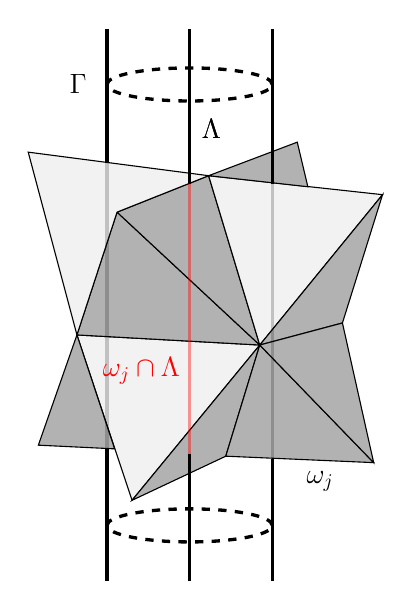
\begin{tikzpicture}[scale=0.7, every node/.style={scale=0.7}]
\pgfmathsetmacro{\factor}{1/sqrt(2)};
\coordinate  (A) at (2,0,-1*\factor);
\coordinate  (B) at (2.2,-1.2,2*\factor);
\coordinate  (C) at (-0.5,1,2*\factor);
\coordinate  (D) at (0.5,-2,2*\factor);
\coordinate  (E) at (0.5,3.5,3*\factor);
\coordinate  (F) at (0.8,2.8,-2*\factor);
\coordinate  (G) at (-1.2,-1,2*\factor);
\coordinate  (H) at (5.7,-0.5,5*\factor);
\coordinate  (I) at (1,-0.25,5*\factor);
\coordinate  (L) at (-2.5,3.2,-2.1*\factor);
\coordinate  (M) at (4.5,3,0*\factor);
\coordinate  (N) at (3.5,0.4,-1*\factor);
\coordinate  (O) at (2,3,-3.5*\factor);
\coordinate  (P) at (2.6,2.6,-2*\factor);
%\draw[->] (0,0) -- (3,0,0) node[right] {$x$};
%\draw[->] (0,0) -- (0,3,0) node[above] {$y$};
%\draw[->] (0,0) -- (0,0,3) node[below left] {$z$};
%\foreach \i in {A,B,C,D}
%\draw[dashed] (0,0)--(\i);
\draw[black, fill=white!90!gray] (A)--(D)--(C)--cycle;
\draw[black,  fill=gray!60!] (A) --(B)--(D)--cycle;
\draw[black, fill=gray!60!] (E) --(C)--(A)--cycle;
\draw[black,   fill=gray!60!] (E) --(F)--(A)--cycle;
\draw[black,    fill=gray!60!] (B) --(A)--(H)--cycle;
\draw[black,    fill=gray!60!] (C) --(G)--(I)--cycle;
\draw[black, fill=white!90!gray] (C) -- (E) -- (F)--(L)--cycle;
\draw[black,  fill=white!90!gray] (A) --(F)--(M)--cycle;
\draw[black,   fill=gray!60!] (A) --(N)--(M)--cycle;
\draw[black,    fill=gray!60!] (A) --(N)--(H)--cycle;
\draw[black,    fill=gray!60!] (F) --(O)--(P)--cycle;
%\draw[-, fill=gray!30!blue, opacity=.2] (E) --(G)--(H)--cycle;
\node [font=\Large, right] at (3, -2.2) {$\omega_j$};


%cylinder Gamma
\draw[dashed, very thick] (1, 5) ellipse (1.5 and 0.3);
\draw[dashed, very thick] (1, -3) ellipse (1.5 and 0.3);
\draw[black, very  thick] (-0.5, 3.6) -- (-0.5, 6);
\draw[black, very thick, opacity=.2] (-0.5, 3.6) -- (-0.5, -1.6);
\draw[black, very  thick] (-0.5, -1.6) -- (-0.5, -4); 
\draw[ very thick] (2.5, 6) -- (2.5, 3.2);
\draw[ very thick, opacity =0.2] (2.5, 3.2) -- (2.5, -1.8);
\draw[very thick] (2.5, -1.8) -- (2.5, -4);
\node [font=\Large, right] at (-1.3, 5) {$\Gamma$};

%centerline \Lambda
\draw[very thick] (1, 6) -- (1, 3.2);
\draw[red, very thick, opacity=.4] (1, 3.2) -- (1, -1.8);
\draw[very thick, ]  (1, -1.7) -- (1, -4);
\node [font=\Large, right] at (1.1, 4.2) {$\Lambda$};
\node [font=\Large, right] at (1.1, 4.2) {$\Lambda$};
\node [font=\Large, right, red] at (-0.7, -0.2) {$\omega _j \cap \Lambda$};
\end{tikzpicture}



%\end{document}
%\caption{Extended patches $\omega_j$.}
%\end{figure}
Moreover, we associate to each patch $\patch$ a shape-regular extended patch (using the classical definition of shape-regularity, see for example \cite{MR2050138}), still denoted by $\omega_j$ for notational simplicity, which is built adding to $\patch$ a sufficient number of elements of $\mathcal{T}_h^{\Omega}$ and we assume that the interiors of the new extended patches $\omega _j$ are still disjoint (see Figure \ref{fig:gamma_generated}). The extended patches $\omega _j$ are built such that they fulfill the conditions meas$(\patch)=\mathcal{O}(H^3)$ and diam$(\Gamma_{\patch\cap \Lambda}\cap \omega_j)=\mathcal{O}(H)$ ($\mathcal{O}(X)$ means $cX \leq \mathcal{O}(X) \leq CX$), where $\Gamma_{\patch\cap \Lambda}$ is the portion of $\Gamma$ with centerline $\patch\cap \Lambda$. The latter assumption is required to ensure that the intersection of $\Gamma_{\patch\cap \Lambda}$ and $\omega_j$ is not too small and it will be needed later on to prove the inf-sup stability of the space $Q_H$ in Lemma \ref{lemma:Lh_infsup}. A representation of this construction in the simple case in which $\omega _j$ is composed just by one tetrahedron is shown in Figure \ref{fig:gamma_generated}.
Thanks to the shape regularity of these extended patches, the following discrete trace inequality holds true for any function $v\in H^1(\omega_j)$, 
\paolo{
\begin{equation}\label{discr_trace_ineq}
\|\trace v\|_{L^2(\Gamma\cap \omega_j)} \leq C_I H^{-\frac 12} \|v\|_{L^2(\omega_j)}
\end{equation}
}
Moreover, $\forall u_h \in X^1_{h,0}(\Omega)$ we have the following average inequality, 
which is a consequence of the definition of $\mtrace$, Jensen inequality, \kent{and the fact that the patches are disjoint}
\begin{multline}\label{eq:avrg_ineq}
\sum _j \|\mtrace u_h\|^2_{L^2(\patch \cap \Lambda),|\DD| }
= \int_{\Lambda} |\DD| \left( \frac{1}{|\DD|} \int_{\DD} \trace u_h \right)^2
\\
\leq \int_{\Lambda} \int_{\DD} (\trace u_h)^2
= \int_{\Gamma} (\trace u_h)^2
= \sum _j \int_{\patch \cap \Gamma} (\trace u_h)^2
= \sum _j \|\trace u_h\|^2_{L^2(\patch \cap \Gamma)}.
\end{multline}
%\kent{Earlier in the paper we always specified the measure, ds, dx etc}

% As shown in \cite[Section III]{burman2014}, we can always choose $\pi_H$ as the $L_2$ orthogonal projection operator from $\Lambda_h$ to $Q_H$ in order to satisfy \eqref{condition_pi_L} and then in practice replace it with any interpolation $\tilde{\pi}_L$ of $\Lambda_h$ in $Q_H$. In particular, for any $\lambda_h \in \Lambda_h$ we define,
% \begin{equation*}
% \tilde{\pi}_L {\ld}_{ _{|\patch}} = M_j^{-1} \sum_{\substack{i: \ K_i \in \mathcal{G}_h, \  K_i \cap \omega_j \neq \emptyset}} {\ld}_{|K_i} \qquad \text{for all $\omega_j$,} 
% \end{equation*}
% being $M_j$ the cardinality of the set $\{i: \ K_i \in \mathcal{G}_h, \  K_i \cap \omega_j \neq \emptyset\}$. These choices lead to the following stabilization 
% \begin{equation}\label{eq:stab}
% s(\ldh, \mdh)= \sum _{K\in \mathcal{G}_{h}} \int_{\partial K\setminus \partial \mathcal{G}_{h}} h \llbracket \ldh \rrbracket \llbracket \mdh \rrbracket,
% \end{equation}
% being $\llbracket \ldh \rrbracket$ the jump of $\ldh$ across the internal faces of $\mathcal{G}_h$.

%\begin{figure}\label{fig:patch}
%\center
%%\documentclass[tikz,border=3mm]{standalone}
%\begin{document}

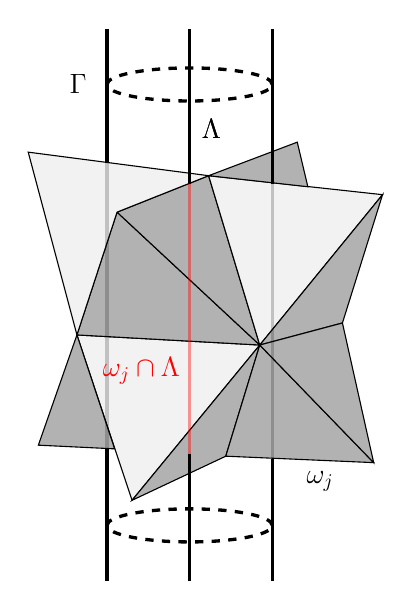
\begin{tikzpicture}[scale=0.7, every node/.style={scale=0.7}]
\pgfmathsetmacro{\factor}{1/sqrt(2)};
\coordinate  (A) at (2,0,-1*\factor);
\coordinate  (B) at (2.2,-1.2,2*\factor);
\coordinate  (C) at (-0.5,1,2*\factor);
\coordinate  (D) at (0.5,-2,2*\factor);
\coordinate  (E) at (0.5,3.5,3*\factor);
\coordinate  (F) at (0.8,2.8,-2*\factor);
\coordinate  (G) at (-1.2,-1,2*\factor);
\coordinate  (H) at (5.7,-0.5,5*\factor);
\coordinate  (I) at (1,-0.25,5*\factor);
\coordinate  (L) at (-2.5,3.2,-2.1*\factor);
\coordinate  (M) at (4.5,3,0*\factor);
\coordinate  (N) at (3.5,0.4,-1*\factor);
\coordinate  (O) at (2,3,-3.5*\factor);
\coordinate  (P) at (2.6,2.6,-2*\factor);
%\draw[->] (0,0) -- (3,0,0) node[right] {$x$};
%\draw[->] (0,0) -- (0,3,0) node[above] {$y$};
%\draw[->] (0,0) -- (0,0,3) node[below left] {$z$};
%\foreach \i in {A,B,C,D}
%\draw[dashed] (0,0)--(\i);
\draw[black, fill=white!90!gray] (A)--(D)--(C)--cycle;
\draw[black,  fill=gray!60!] (A) --(B)--(D)--cycle;
\draw[black, fill=gray!60!] (E) --(C)--(A)--cycle;
\draw[black,   fill=gray!60!] (E) --(F)--(A)--cycle;
\draw[black,    fill=gray!60!] (B) --(A)--(H)--cycle;
\draw[black,    fill=gray!60!] (C) --(G)--(I)--cycle;
\draw[black, fill=white!90!gray] (C) -- (E) -- (F)--(L)--cycle;
\draw[black,  fill=white!90!gray] (A) --(F)--(M)--cycle;
\draw[black,   fill=gray!60!] (A) --(N)--(M)--cycle;
\draw[black,    fill=gray!60!] (A) --(N)--(H)--cycle;
\draw[black,    fill=gray!60!] (F) --(O)--(P)--cycle;
%\draw[-, fill=gray!30!blue, opacity=.2] (E) --(G)--(H)--cycle;
\node [font=\Large, right] at (3, -2.2) {$\omega_j$};


%cylinder Gamma
\draw[dashed, very thick] (1, 5) ellipse (1.5 and 0.3);
\draw[dashed, very thick] (1, -3) ellipse (1.5 and 0.3);
\draw[black, very  thick] (-0.5, 3.6) -- (-0.5, 6);
\draw[black, very thick, opacity=.2] (-0.5, 3.6) -- (-0.5, -1.6);
\draw[black, very  thick] (-0.5, -1.6) -- (-0.5, -4); 
\draw[ very thick] (2.5, 6) -- (2.5, 3.2);
\draw[ very thick, opacity =0.2] (2.5, 3.2) -- (2.5, -1.8);
\draw[very thick] (2.5, -1.8) -- (2.5, -4);
\node [font=\Large, right] at (-1.3, 5) {$\Gamma$};

%centerline \Lambda
\draw[very thick] (1, 6) -- (1, 3.2);
\draw[red, very thick, opacity=.4] (1, 3.2) -- (1, -1.8);
\draw[very thick, ]  (1, -1.7) -- (1, -4);
\node [font=\Large, right] at (1.1, 4.2) {$\Lambda$};
\node [font=\Large, right] at (1.1, 4.2) {$\Lambda$};
\node [font=\Large, right, red] at (-0.7, -0.2) {$\omega _j \cap \Lambda$};
\end{tikzpicture}



%\end{document}
%\caption{Extended patches $\omega_j$.}
%\end{figure}

\begin{figure}\label{fig:gamma_generated}
\centering
\includegraphics[width=0.32\textwidth]{./graphics/ext_patch.tex}
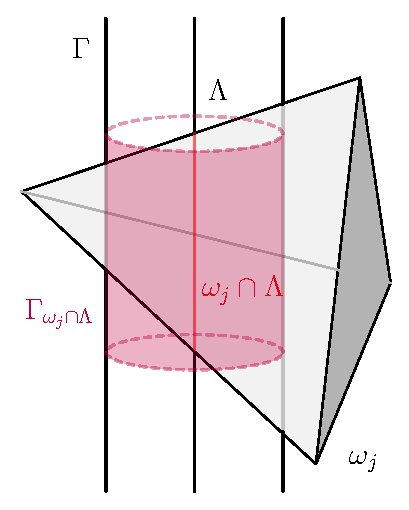
\includegraphics[width=0.32\textwidth]{./graphics/gamma_generated}
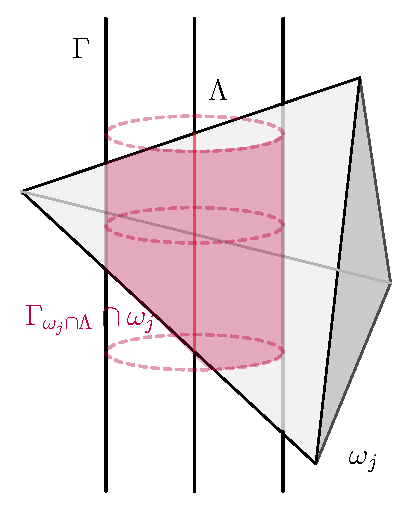
\includegraphics[width=0.32\textwidth]{./graphics/intersection}
\caption{
(Left) Extended patches $\omega_j$. (Middle)
$\Gamma_{\omega_j \cap \Lambda}$, the portion of $\Gamma$ generated by $\omega_j \cap \Lambda$. (Right) the intersection between $\Gamma_{\omega_j \cap \Lambda}$ and $\omega_j$. Here for simplicity $\omega_j$ is represented as a single tetrahedron but actually it is a collection of tetrahedra as shown in left panel.}
\end{figure}

We are now ready to prove that the space $Q_H$ is inf-sup stable. 
\begin{lemma}\label{lemma:Lh_infsup}
The space $Q_H$ is inf-sup stable, 
namely there exists $\beta >0$ such that
\begin{equation*}
\sup_{\substack{v_h \in X_{h,0}^1(\Omega),\\ \vdfh \in X_{\fkh,0}^1(\Lambda)}} \frac{\left(\mtrace v_h - \vdfh, {\md} _H\right)_{\Lambda, |\DD|}}{\vertiii{[v_h, \vdfh]}} \geq \beta \|{\md}_H\|_{H^{-\frac 12}(\Lambda)} \quad \forall {\md}_H \in Q_H.
\end{equation*} 
\end{lemma}

\begin{proof}
We choose $\vdfh=0$ and we prove that
\begin{equation*} 
\sup_{v_h \in X_{h,0}^1(\Omega)} \frac{\left(\mtrace v_h ,{\md}_H\right)_{\Lambda, |\DD|}}{\|v_h\|_{H^1(\Omega)}} \geq \beta \|{\md}_H\|_{H^{-\frac 12}(\Lambda)}.
\end{equation*} 
Proving the last inequality is equivalent to finding the Fortin operator $\pi_F: H^1_0(\Omega) \rightarrow X_{h,0}^1(\Omega)$, such that 
\begin{gather}
\left(\mtrace v - \mtrace \pi _F v  , {\md}_H\right)_{\Lambda, |\DD|}=0, \quad \forall v\in H^1_0(\Omega), \, {\md}_H \in Q_H\,,
\\
\label{eq:cont_Fortin}
\|\pi_F v\|_{H^1(\Omega)} \leq C \|v\|_{H^1(\Omega)}\,.
\end{gather} 

We define
\begin{equation*}
\pi_F v = I_h v + \sum _j \alpha _j \varphi _j \qquad \text{with }\alpha_j =\frac{\int_{\patch \cap \Lambda}|\DD| (\mtrace v-\mtrace I_h v)}{\int_{\patch \cap \Lambda}|\DD|\mtrace \varphi _j}
\end{equation*}
where $I_h: H^1(\Omega) \rightarrow X_{h,0}^1(\Omega)$ denotes an $H^1(\Omega)$-stable interpolant
and $\varphi_j \in X_{h,0}^1(\Omega)$ is such that supp$(\varphi_j)\subset \omega_j$, supp$(\trace \varphi _j) \subset \Gamma_{\patch\cap \Lambda}\cap \omega_j$, $\varphi_j =0$ on $\partial \omega _j$ and 
\begin{equation}\label{phi_properties}
\int_{\patch\cap \Lambda}|\DD|\mtrace \varphi_j=\mathcal{O}(H) \text{ and } \|\nabla \varphi _j\|_{L^2(\omega _j)}=\mathcal{O}(1). 
\end{equation}
We notice that supp$(\trace \varphi_j) \subset \Gamma_{\patch\cap \Lambda}\cap \omega_j$ ensures that $\mtrace \varphi_j \subset \omega_j\cap \Lambda$. Therefore, since the interiors of $\omega_j\cap \Lambda$  are disjoint and $\varphi _j = 0 $ on $\partial \omega_j$,  the functions $\mtrace \varphi_j\, \forall j$ have all disjoint supports. Provided $H$ is sufficiently larger that $h$, the functions $\varphi _j$ and their traces $\trace \varphi _j$ have a sufficiently large support thanks to the fact that $\mathrm{meas}(\patch) = \mathcal{O}(H^3)$ and $\mathrm{diam}(\Gamma_{\patch\cap \Lambda} \cap \omega_j)=\mathcal{O}(H)$.
Owing to these properties it is possible to satisfy \eqref{phi_properties}. 
\kent{Then, by construction,}
\begin{multline*}
\left(\mtrace v - \mtrace \pi _F v  , {\md}_H\right)_{\Lambda, |\DD|} = \sum _j \int_{\patch\cap \Lambda} |\DD |\left[ \mtrace v-\mtrace I_h v-\sum _i \alpha_i \mtrace \varphi _i \right]{\md}_H \\
=\sum _j \int_{\patch\cap \Lambda}|\DD| \left[ \mtrace v-\mtrace I_h v-\alpha_j \mtrace \varphi _j \right]{\md}_H
\\
% =\sum _j \left[\int_{\patch\cap \Lambda} |\DD| (\mtrace v-\mtrace  I_h v) {\md}_H - \frac{\int_{\patch\cap \Lambda} |\DD| (\mtrace v-\mtrace I_h v)}{\int_{\patch\cap \Lambda}|\DD|\mtrace \varphi _j} \int_{\patch\cap \Lambda} |\DD|\mtrace \varphi _j{\md}_H\right]
% \\ 
=\sum _j \left[\int_{\patch\cap \Lambda} |\DD| (\mtrace v-\mtrace  I_h v) {\md}_H
-[\int_{\patch\cap \Lambda} |\DD| (\mtrace v-\mtrace  I_h v) {\md}_H \right]=0.
\end{multline*}
Concerning the continuity of $\pi_F$, we exploit the assumptions that the interiors of $\patch$ are disjoint, $\mathrm{supp}(\varphi _j) \subset \patch$ and the $H^1$-stability of $I_h$ to show that
\begin{equation*}
\|\nabla \pi_F v \|_{L^2(\Omega)} 
% \leq \|\nabla I_h v\|_{L^2(\Omega)} + \left(\sum_j\alpha_j^2\|\nabla \varphi _j\|^2_{L^2(\omega_j)}\right)^{\frac 12}
\leq C \|\nabla  v\|_{L^2(\Omega)} + \left(\sum_j\alpha_j^2\|\nabla \varphi _j\|^2_{L^2(\omega_j)}\right)^{\frac 12}\,.
\end{equation*}
For the second term,
using that $\|\nabla \varphi _j\|_{{L^2(\omega_j)}}=\mathcal{O}(1)$, 
$\int_{\patch\cap \Lambda}|\DD|\mtrace \varphi_j=\mathcal{O}(H)$ and that
$|\patch\cap \Lambda| \leq cH$,
\kent{exploiting Jensen's average inequality} \eqref{eq:avrg_ineq} 
and trace inequality \eqref{discr_trace_ineq},
and finally applying the approximation properties of $I_h$,
the following upper bound holds true
\paolo{(where all the constants have been condensed into $C$),}
\begin{multline*}
\sum_j \alpha_j ^2\|\nabla \varphi _j\|^2_{L^2(\omega_j)}
\leq C \sum_j \frac{\left(\int_{\patch\cap \Lambda} |\DD| (\mtrace v-\mtrace I_h v)\right)^2}{\left(\int_{\patch\cap \Lambda}|\DD|\mtrace \varphi_j \right)^2}
\\
% \leq \frac {C}{H^2} \sum_j \left(\int_{\patch\cap \Lambda} |\DD| (\mtrace v-\mtrace I_hv)\right)^2
\leq \frac {C}{H^2} \sum_j |\patch\cap \Lambda| \int_{\patch\cap \Lambda} |\DD|^2(\mtrace v-\mtrace I_h v)^2
\\
\leq \frac {C}{H} \sum_j \| \mtrace (v-I_h v)\|^2_{L^2(\patch\cap \Lambda), |\DD|}
\leq \frac {C}{H} \sum_j \| \trace(v-I_h v)\|^2_{L^2(\omega _j\cap \Gamma)}  
\\
\leq \frac {C}{H^2} \sum_j  \| v-I_h v\|^2_{L^2(\omega_j)} 
\leq C \frac {1}{H^2}  \| v-I_h v\|^2_{L^2(\Omega)} 
\leq C \|\nabla  v\|^2_{L^2(\Omega)}
\end{multline*}
that is the $H^1$-stability of $\pi_F$. We notice that the constant in the inequality \eqref{eq:cont_Fortin} is independent of how $\Lambda$  cuts the elements of the mesh $\mathcal{T}_h^{\Omega}$.
\end{proof}

For the second assumption of Lemma \ref{lemma23burman}, we recall that $b(v_h,\mdh)$ is continuous \kent{with respect to the norms} $\vertiii{v_h},\,\|\mdh\|_{L^2(\Lambda)}$. 
Using Lemma \ref{lemma:Lh_infsup}, and in particular the existence of a Fortin projector,
there exists a constant $\beta$ such that 
(the proof is \miro{analogous} to the one of Lemma 2.1 in \cite{burman2014})
\begin{equation}\label{relax_infsup}
\beta \|\mdh\|_{H^{-\frac12}(\Lambda)} \leq \sup\limits_{v_h \in X_h} \frac{b(v_h,\mdh)}{\vertiii{v_h}} + \|\mdh-\pi_H \mdh\|_{L^2(\Lambda)}, \quad \forall \mdh \in Q_h\,.
\end{equation}
We define $\pi_H = \sum_j \pi_H^j\,: L^2(\Lambda) \rightarrow Q_H$, 
where $\pi_H^j$ is the operator
\begin{equation}\label{eq:projector}
\pi_H^j w_{|\patch \cap \Lambda} =\frac{1}{|\Gamma_{\patch\cap \Lambda}|}\int_{\patch\cap \Lambda}|\DD| w\quad \forall j.
\end{equation}   
Since $\cup_j \omega_j \cap \Lambda  = \Lambda$ and $\omega_j \cap \Lambda$ are not overlapping,
we obtain that $\pi_H$ is an orthogonal projection, namely $(w-\pi_H w,\pi_H w)=0$.
Moreover, for any $w \in L^2(\Lambda)$ the following Poincarè inequality holds true, see for example \cite[Corollary B.65]{MR2050138},
\begin{equation}\label{disc_poincare_ineq}
\|w - \pi_H w\|_{L^2(\omega_j\cap\Lambda),|\DD|} \leq C_P H \|\partial_s w\|_{L^2(\omega_j\cap\Lambda),|\DD|}\,.
\end{equation}
We consider the following stabilization operator
\begin{equation}\label{eq:stab}
s_h(\ldh, \mdh)= \sum _{K\in \mathcal{G}_{h}} \int_{\partial K\setminus \partial \mathcal{G}_{h}} h \llbracket \ldh \rrbracket \llbracket \mdh \rrbracket,
\end{equation}
being $\llbracket \ldh \rrbracket$ the jump of $\ldh$ across the internal faces of $\mathcal{G}_h$.
Then, we use the result of \cite{burman2014}, Section III to show that
\begin{equation*}
    \|\mdh-\pi_H \mdh\|_{L^2(\Lambda)} \leq C s_h(\mdh, \mdh)\,,
\end{equation*}
which combined with \eqref{relax_infsup} shows that the second assumption of Lemma \ref{lemma23burman} holds true.

The third step of the analysis consists of showing that \eqref{stab_coercivity} and \eqref{stab_stability} are satisfied. 
We introduce the following discrete norms
\begin{equation*}
\|\, \lambda \,\|_{\pm \frac 12, h, \Lambda} = \|h^{\mp\frac 12} \lambda\|_{L^2(\Lambda)},
\end{equation*}
recalling that $h$ is the mesh size of $\mathcal{T}^\Omega_{h}$. We equip the space $X_h$ with the discrete norm
\begin{equation*}
\vertiii{[u_h, \udfh]}^2_{X_h}
= \|u_h\|^2_{H^1(\Omega)}+\|\udfh\|^2_{H^1(\Lambda),|\D|} + \|\mtrace u_h - \udfh\|^2_{\frac 12, h, \Lambda, |\DD|},
\end{equation*}
and the space $Q_H$ with the $L^2$ norm $\|{\md}_H \|_{L^2(\Lambda)}$.

Also, the function $\xi_h([v_h, \vdfh]) \in Q_H \subset Q_h \subset L^2(\Lambda)$ is defined as follows
\begin{equation*}
{\xi_h}_{|\patch\cap \Lambda}=\frac{\delta}{H} \pi_H(\mtrace u_h-\udfh)_{|\patch \cap \Lambda}.
\end{equation*}
where $\delta$ is an arbitrarily small parameter. Then the following result holds true. 
\begin{lemma}
Given $\pi_H,\ s_h(\cdot,\cdot), \ \xi_h$ defined above, 
choosing $\delta$ small enough,
the inequalities \eqref{stab_coercivity} and \eqref{stab_stability} are satisfied.
\end{lemma}
\begin{proof} 
Concerning the coercivity property \eqref{stab_coercivity}, we show that $\forall [u_h, \udfh]$, there exists $\xi_h \in Q_h$ such that,
\begin{equation*}
(u_h,u_h)_{H^1(\Omega)}+ (\udfh, \udfh)_{H^1(\Lambda), |\D|} +   (\mtrace u_h - \udfh, \xi_h)_{\Lambda,|\DD|} \geq \alpha_{\xi}\vertiii{[u_h, \udfh]}^2_{X_h}.
\end{equation*}
Using the definitions of $\pi_H$ and $\xi_h([u_h, \udfh])$ previously presented and recalling that $\xi_h\in Q_H \subset Q_h$, we obtain
\begin{multline*}
\left( \mtrace u_h - \udfh, \xi _h \right)_{\Lambda,|\DD|} 
% = \sum_j \int_{\patch\cap \Lambda} |\DD|(\mtrace u_h - \udfh)\xi_h
= \frac{\delta}{H}\sum_j \pi_H^j( \mtrace u_h - \udfh)\int_{\patch\cap \Lambda} |\DD|(\mtrace u_h - \udfh)
\\
= \frac{\delta}{H} \sum_j \int_{\patch\cap \Lambda}|\DD| (\pi_H( \mtrace u_h - \udfh) )^2
= \frac{\delta}{H}\sum_j \|\pi_H( \mtrace u_h - \udfh)\|_{L^2(\patch\cap \Lambda),|\DD|}^2
\\
= \frac{\delta}{H} \sum_j \left( \|\mtrace u_h - \udfh\|^2_{L^2(\patch\cap \Lambda),|\DD|} - \|(\pi_H-\mathcal{I})(\mtrace u_h - \udfh)\|^2_{L^2(\patch\cap \Lambda),|\DD|} \right) 
\\ 
\geq \frac{\delta}{H} \sum_j \left(
\|\mtrace u_h-\udfh\|^2_{L^2(\patch\cap \Lambda),|\DD|}
- \|(\pi_H - \mathcal{I})\mtrace u_h\|^2_{L^2(\patch\cap \Lambda), |\DD|} \right.
\\
\left.- \|(\pi_H - \mathcal{I})\udfh\|^2_{L^2(\patch\cap \Lambda),|\DD|} \right). 
\end{multline*}
Now, we seek for an upper bound of the second and third (negative) terms of the last inequality.
For the second term, we apply the additional assumption that the operators $\mtrace$ and $\partial_s$ commute. This is true if the cross section $\D$ does not depend on the arclength $s$.
\paolo{
Then, we use the Poincar\'e inequality \eqref{disc_poincare_ineq}, the average inequality \eqref{eq:avrg_ineq} and the trace inequality \eqref{discr_trace_ineq} to show that,
\begin{multline*}
\sum _j  \|(\pi_H - \mathcal{I})\mtrace u_h\|^2_{L^2(\patch\cap \Lambda),|\DD|} 
% \leq C_P^2 H^2 \sum _j \|\partial_s \mtrace u_h\|_{L^2(\patch\cap \Lambda),|\DD|}^2
\leq C_P^2 H^2 \sum _j \|\mtrace \partial_s  u_h\|_{L^2(\patch\cap \Lambda),|\DD|}^2
\\
\leq C_P^2 H^2 \sum _j \|\trace \partial_s u_h\|_{L^2(\omega _j \cap \Gamma)}^2
\leq C_P^2 C_I^2 H \sum _j \|\nabla u_h\|_{L^2(\omega _j)}^2.
\end{multline*}
% old version, wrong
% \begin{multline*}
% \sum _j  \|(\pi_H - \mathcal{I})\mtrace u_h\|^2_{L^2(\patch\cap \Lambda),|\DD|} =\sum _j \int _{\patch \cap \Lambda} |\DD| (\pi_H \mtrace u_h- \mtrace u_h)^2
% \\
% (\text{Average inequality \eqref{eq:avrg_ineq}}) \leq \sum _j  \int_{\omega _j \cap \Gamma} (\ext \pi_H \mtrace u_h -\trace u_h)^2 
% \\
% (\text{trace inequality \eqref{discr_trace_ineq}}) \leq \sum _j  \frac 1H \int_{\omega_j}(\mathcal{E}_{\patch} \pi_H \mtrace u_h - u_h)^2 
% \\ 
% (\text{Poincare, see \cite[Corollary B.65]{MR2050138}})\leq \sum _j  H c_P ^2 \|\nabla u_h\|^2_{L^2(\omega _j)}.
% \end{multline*}
% \kent{Is it $C_P$}
% \paolo{For the third term we observe that since $H \lesssim 1$, there exists a constant $C$ 
% such that $C_P^2 H|\DD| \leq C |\D|$.
For the third term, the following upper bound holds true,
\begin{multline*}
\sum _j \|(\pi_H - \mathcal{I})\udfh\|^2_{L^2(\patch\cap \Lambda),|\DD|} \leq C_P^2 H^2 \sum _j \|\partial_s \udfh\|_{L^2(\patch\cap \Lambda),|\DD|}^2
\\
\leq C_P^2 H^2 \frac{\max |\DD|}{\min |\D|} \sum _j \|\partial_s \udfh\|_{L^2(\patch\cap \Lambda),|\D|}^2.
\end{multline*}
%{\color{red} N.B. we are using a kind of weigthed Poincare inequality, check... I think it should work because I can do something like this
%\begin{multline*}
%\int_{\patch \cap \Lambda} |\DD| u^2 \leq 
%max |\DD| \int_{\patch \cap \Lambda} u^2 \leq
%max |\DD| \int_{\patch \cap \Lambda} (\nabla u)^2 =
%\frac{max |\DD|}{min|\DD|} min|\DD| \int_{\patch \cap \Lambda} (\nabla u)^2 \leq\\
%\frac{max |\DD|}{min|\DD|}  \int_{\patch \cap \Lambda} |\DD| (\nabla u)^2 
%\end{multline*}
%}\\
Combining the last three inequalities, reminding that $c_h h\leq H \leq c_H^{-1}h$, 
we obtain
\begin{multline*}
a([u_h, \udfh],[u_h, \udfh] ) + b([u_h, \udfh], \xi_h([u_h, \udfh]))
\geq (1-\delta C_P^2 C_I^2) \|\nabla u_h\|^2_{L^2(\Omega)} 
\\
+ \left(1- \delta C_P^2 H \frac{\max |\DD|}{\min |\D|}\right) \|\partial_s \udfh\|^2_{L^2(\Lambda), |\D|}
+\delta c_H  \|\mtrace u_h-\udfh\|^2_{\frac 12,h,\Lambda, |\DD|}
\end{multline*}
and choosing $\delta=\frac{1}{2}\min\left[(C_P^2 C_I^2)^{-1}, \left(C_P^2 H \frac{\max |\DD|}{\min |\D|}\right)^{-1}\right]$ we obtain the desired inequality.
Concerning inequality \eqref{stab_stability}, the proof is analogous to the one in \cite{burman2014}.}
\end{proof}

% \begin{remark}
% We notice that if we choose $Q_h=X_{h',0}^1(\Lambda)$, the constant in the inf-sup inequality  \eqref{eq:infsup_discrete} depends on the mesh size $h'$. Indeed,
% \begin{multline}
% \sup_{\substack{v_h \in X_{h,0}^1(\Omega),\\ \vdfh \in X_{h',0}^1(\Lambda)}} \frac{\left(\mtrace v_h - \vdfh, {\md} _H\right)_{\Lambda, |\DD|}}{\vertiii{[v_h, \vdfh]}}
% \geq \sup_{\substack{\vdfh \in X_{h',0}^1(\Lambda)}} \frac{\left(- \vdfh, {\md} _H\right)_{\Lambda, |\DD|}}{\|\vdfh\|_{H^1(\Lambda)}}
% \geq \frac{{\|\md} _H\|^2_{L^2(\Lambda)}}{\|\vdfh\|_{H^1(\Lambda)}} \\
% ( \text{inverse inequality} )\geq \frac{{h'}^2}{c_I} \|{\md}_H\|_{L^2(\Lambda)}
% \geq  \frac{{h'}^2}{c_I} \|{\md}_H\|_{H^{-\frac 12},(\Lambda)}
% \end{multline}
% being $c_I$ the constant in the inverse inequality
% \begin{equation*}
% \|{\md}_H\|_{H^1(\Lambda)} \leq \frac{c_I} {{h'}^2} \|{\md}_H\|_{L^2(\Lambda)}. 
% \end{equation*}
% \end{remark}


%>>>>>>>>>>>>>>>>>>>>>>>>>>>>>>>>>>>>>>>>>>>>>>>>>>
\section{A benchmark problem with analytical solution}

Let $\Omega=[0,1]^3$, $\Lambda=\{x=\tfrac{1}{2}\}\times \{y=\tfrac{1}{2}\} \times [0,1] $
and $\Omega_{\ominus}=[\tfrac{1}{4}, \tfrac{3}{4}]\times [\tfrac{1}{4}, \tfrac{3}{4}]\times [0, 1]$.
%Finally we let $\DD$ be the cross section of the virtual interface $\Gamma=\partial \Sigma$.
As a benchmark for the two formulations we consider the following coupled problems
%
\begin{subequations}\label{benchmark}
\begin{align}
\label{benchm_3d}
-\Delta u=f \quad &\text{in $\Omega$},\\
\label{benchm_1d}
-d_{zz}^2 \ud =\avrd{g} \quad &\text{on $\Lambda$},\\
u=u_b \quad &\text{on $\partial \Omega$},
\end{align}
\end{subequations}
where for formulation \eqref{eq:problem1} the mix-dimensional coupling constraint reads
\begin{equation}
  \label{eq:couple_1}
\trace{u} - \ext{\ud} = q_1\quad\text{ on }\Gamma,
\end{equation}
while for \eqref{eq:problem2} we set
\begin{equation}
    \label{eq:couple_2}
\avrc{u} - \ud = \avrc{q}_2\quad\text{ on }\Lambda.
\end{equation}
%
In \eqref{benchmark}-\eqref{eq:couple_2} the right-hand sides shall be defined as 
\begin{eqnarray*}
  &f=8\pi ^2 \sin (2\pi x) \sin (2\pi y),\quad &\avrd{g}={\pi ^2}\sin \left({\pi z}\right),\quad u_b=\sin (2\pi x) \sin (2\pi y),\\
  &q_1=\sin (2\pi x) \sin (2\pi y) - \sin \left({\pi z}\right),\quad &\avrc{q}_2=-\sin \left({\pi z}\right).
\end{eqnarray*}

The exact solution of \eqref{benchmark}, regardless of the coupling constraint,
is given by
%
\begin{equation}
\label{benchm_sol3d-1d}
u=\sin (2\pi x) \sin (2\pi y),
\quad
%\ud=1+\exp(-z).
\ud=\sin \left({\pi z}\right).
\end{equation}
%
Let us notice that $\ud$ satisfies homogeneous Dirichlet conditions at the boundary of $\Lambda$.
Moreover, the solution \eqref{benchm_sol3d-1d} satisfies on $\Gamma$ the relation
\begin{equation}\label{benchm_flux}
\nabla u \cdot \textbf{n}_{\oplus}=d_z \ud n_{\oplus,z}=0,
\end{equation}
with $n_{\oplus,z}$ the $z-$component of the normal unit vector to $\Gamma$.

% in the case in which the starting 3D-3D problem is
% \begin{subequations}\label{eq:dirneu_simple}
% \begin{align}
% - \Delta \up  &= f  && \text{ in } \Omega_{\oplus},\\
% - \Delta \uf &= g  && \text{ in } \Omega_{\ominus},\\
% -\nabla \uf \cdot \nn_{\ominus} &= -\nabla \up \cdot \nn_{\ominus}  && \text{ on } \Gamma,\\
% \uf - \up &= q_i  && \text{ on }  \Gamma,\\
% \up &= \paolo{u_b} && \text{ on } \partial \Omega,
% \end{align}
% \end{subequations}
% Therefore the reduced problems in \eqref{eq:problem1} and
% \eqref{eq:problem2} become respectively
% %
% \begin{subequations}\label{eq:problem1_simple}
% \begin{align}
% \label{eq:problem1_simple_eq1}
% &(\nabla u,\nabla v)_{L^2(\Omega)} + |{\cal D}|(d_s \ud,d_s \vd)_{L^2(\Lambda)} 
% + \langle \trace{v}  - \ext{\vd}, \lambda \rangle_\Gamma
% \\
% \nonumber
% &\qquad\qquad= (f,v)_{L^2(\Omega)} + |{\cal D}| (\avrd{g},\vd)_{L^2(\Lambda)}
% \quad \forall v \in H^1_0(\Omega), \ \vd \in H^1_0(\Lambda)
% \\
% \label{eq:problem1_simple_eq2}
% &   \langle \trace{u} - \ext{\ud} , \mu \rangle_\Gamma =  \langle q_1 , \mu \rangle_\Gamma
% \quad \forall \mu \in H^{-\frac12}(\Gamma)
% \end{align}
% \end{subequations}
% % and
% \begin{subequations}\label{eq:problem2_simple}
%   \begin{align}
%     \label{eq:problem2_simple_eq1}
% &(\nabla u,\nabla v)_{L^2(\Omega)} + |{\cal D}|(d_s \ud,d_s \vd)_{L^2(\Lambda)} 
% + |{\partial \cal D}| \langle \avrc{v} - \vd, \ld \rangle_{H^{-\frac12}(\Lambda)} 
% \\
% \nonumber
% &\qquad\qquad= (f,v)_{L^2(\Omega)} + |{\cal D}| (\avrd{g}, \vd)_{L^2(\Lambda)}
% \quad \forall v \in H^1_0(\Omega), \ \vd \in H^1_0(\Lambda)
% \\
% \label{eq:problem2_simple_eq2}
% &  |\partial {\cal D}| \langle \avrc{u} -  \ud, \md \rangle_{H^{-\frac12}(\Lambda)} =
% |\partial {\cal D}| \langle \avrc{q_2}, \md \rangle_{H^{-\frac12}(\Lambda)}
% \quad \forall \md \in H^{-\frac12}(\Lambda)\,.
% \end{align}
% \end{subequations}

\paolo{We prove that the solution of \eqref{benchmark} is equivalent to the one of \eqref{eq:problem2}.}
Precisely, we prove that \eqref{benchm_sol3d-1d} is the solution of
\eqref{eq:problem2}. Using the integration by part formula and homogeneous
boundary conditions on $\Omega$ and $\Lambda$, from \eqref{eq:problem2} we have
\begin{align*}
&-(\Delta u, v)_{L^2(\Omega)} - |{\cal D}|(d^2_{ss} \ud, \vd)_{L^2(\Lambda)} 
+ |{\cal D}|\langle \avrc{v}  - \vd, \ld \rangle_\Lambda
\\
\nonumber
&\qquad\qquad= (f,v)_{L^2(\Omega)} + |{\cal D}| (\avrd{g},\vd)_{L^2(\Lambda)}
\quad \forall v \in H^1_0(\Omega), \vd \in H^1(\Lambda).
\end{align*}
Since $\ld=0$ and the first of \eqref{benchm_sol3d-1d} satisfies \eqref{benchm_3d} and the second satisfies \eqref{benchm_1d}, we have that
\begin{align*}
-(\Delta u, v)_{L^2(\Omega)} =  (f,v)_{L^2(\Omega)}, 
\\
-|{\partial \cal D}|(d^2_{ss} \ud, \vd)_{L^2(\Lambda)}  = |{\cal D}| (\avrd{g},\vd)_{L^2(\Lambda)}.
\end{align*}
Thus \eqref{benchm_sol3d-1d} satisfy equations \eqref{eq:problem2a}, \eqref{eq:problem2b}.
The fact that the solution satisfy \eqref{eq:problem2c} follows from \eqref{eq:couple_2}.

We can prove in a similar way that \eqref{benchm_sol3d-1d}, with $\lambda=0$
satisfy \eqref{eq:problem1}. Note in particular that $q_1$ is such that
$\trace{u} - \ext{\ud} = q_1$ on $\Gamma$.

\subsection{Numerical experiments. $\mathcal{T}^{\Omega}_h$ conforming to $\Gamma$}\label{sec:experiment_conform}
Using the benchmark problem \eqref{benchmark} we now investigate convergence
properties of the two formulations. To this end we consider a \emph{uniform} mesh
of $\mathcal{T}^{\Omega}_h$ of $\Omega$ consisting of tetrahedra with diameter $h$.
Further, the discretization shall be geometrically \emph{conforming} to both $\Lambda$
and $\Gamma$ such that the meshes $\mathcal{T}^{\Gamma}_h$, $\mathcal{T}^{\Lambda}_h$
are made up of facets and edges of $\mathcal{T}^{\Omega}_h$ respectively, cf. Figure \ref{fig:mesh}
for illustration.


\begin{figure}
 \centering
 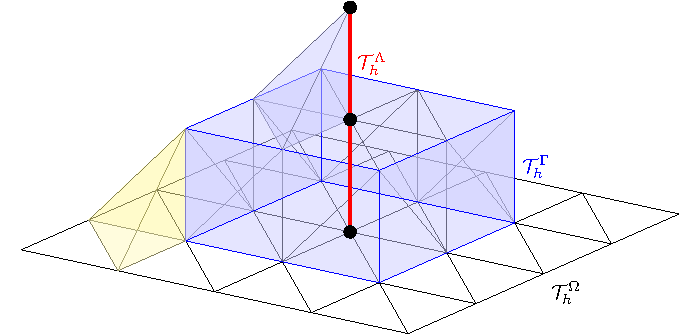
\includegraphics[width=0.45\textwidth]{graphics/conform_mesh.pdf}
 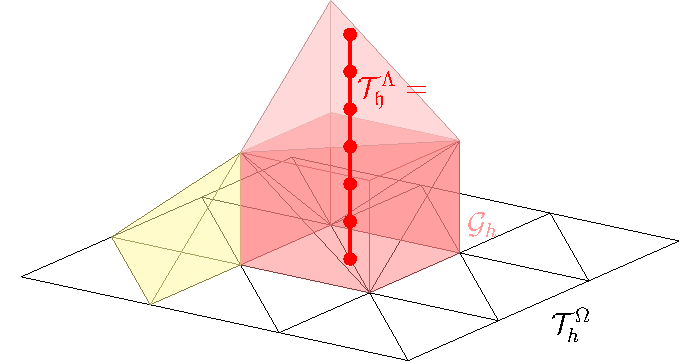
\includegraphics[width=0.45\textwidth]{graphics/nonconform_mesh.pdf} 
 \vspace{-10pt}
 \captionof{figure}{
   (Left)
$\Lambda$ and $\Gamma$ conforming discretization of $\Omega$
   used for \eqref{eq:problem1} and \eqref{eq:problem2}.
   (Right) Sample discretization of the benchmark geometry in the non-conforming case for \eqref{eq:problem2}. 
 }
\label{fig:mesh}
\end{figure}

\begin{table}
  \scriptsize{
  \begin{center}
    \begin{tabular}{l|llll}
\hline
\multicolumn{5}{c}{\textcolor{blue}{$\mathcal{T}^{\Omega}_h$ conforming to $\Gamma$, $\Lambda$}}\\
\hline
    $h^{-1}$ & $\norm{u-u_h}_{H^1(\Omega)}$ & $\norm{\ud-\udh}_{H^1(\Lambda)}$ & $\norm{\lambda-\lambda_h}_{H^{-1/2}(\Gamma)}$ & $\norm{\lambda-\lambda_h}_{L^2(\Gamma)}$\\
      \hline
4  & 3.4E0(--)    & 5.3E-1(--)   & 2.9E0(--)    &8.7E0(--)    \\
8  & 1.7E0(0.99)  & 2.6E-1(1.06) & 6.1E-1(2.25) &1.9E0(2.21)  \\
16 & 8.7E-1(0.99) & 1.3E-1(1.02) & 1.4E-1(2.13) &4.7E-1(1.99) \\
32 & 4.4E-1(1.00) & 6.3E-2(1.00) & 3.4E-2(2.03) &1.3E-1(1.80) \\
64 & 2.2E-1(1.00) & 3.1E-2(1.00) & 8.6E-3(2.00) &4.2E-2(1.68) \\
\hline
$h^{-1}$ & $\norm{u-u_h}_{H^1(\Omega)}$ & $\norm{\ud-u_{\odot}}_{H^1(\Lambda)}$ & $\norm{\ld-\ldh}_{H^{-1/2}(\Lambda)}$ & $\norm{\ld-\ldh}_{L^2(\Lambda)}$\\
\hline
4   & 3.1E0(--)    & 5.4E-1(--)   & 4.4E-2(--)   & 7.8E-2(--)  \\
8   & 1.7E0(0.87)  & 2.6E-1(1.06) & 1.1E-2(2.01) & 1.9E-2(2.01)\\
16  & 8.6E-1(0.96) & 1.3E-1(1.02) & 2.7E-3(2.01) & 4.8E-3(2.02)\\
32  & 4.4E-1(0.99) & 6.3E-2(1.00) & 6.7E-4(2.01) & 1.2E-3(2.01)\\
64  & 2.2E-1(1.00) & 3.1E-2(1.00) & 1.7E-4(2.01) & 3.0E-4(2.01)\\
128 & 1.1E-1(1.00) & 1.6E-2(1.00) & 4.1E-5(2.01) & 7.4E-5(2.00)\\
\hline
\multicolumn{5}{c}{\textcolor{red}{$\mathcal{T}^{\Omega}_h$ non conforming to $\Gamma$, $\Lambda$}}\\
%    \begin{tabular}{l|lll}
\hline
    $h^{-1}$ & $\norm{u-u_h}_{H^1(\Omega)}$ & $\norm{\ud-u_{\odot\mathfrak{h}}}_{H^1(\Lambda)}$ & \multicolumn{2}{c}{$\norm{\ld-\ldh}_{L^2(\mathcal{G}_h)}$}\\
      \hline
5   & 2.6E0(--)    & 2.3E-1(--)   & \multicolumn{2}{c}{1.7E-1(--)} \\ 
9   & 1.5E0(0.84)  & 9.4E-2(1.42) & \multicolumn{2}{c}{7.1E-2(1.36)}\\
17  & 8.1E-1(0.94) & 4.3E-2(1.18) & \multicolumn{2}{c}{2.9E-2(1.37)}\\
33  & 4.2E-1(0.98) & 2.1E-2(1.06) & \multicolumn{2}{c}{7.9E-3(1.91)}\\
65  & 2.1E-1(0.99) & 1.1E-2(1.02) & \multicolumn{2}{c}{2.6E-3(1.64)}\\
129 & 1.1E-1(1.00) & 5.2E-3(1.01) & \multicolumn{2}{c}{8.5E-4(1.61)}\\
\hline
    \end{tabular}
  \end{center}    
  }
  \captionof{table}{Error convergence on a benchmark problem \eqref{benchmark}.
    (Top) problem \eqref{eq:problem1}, (middle) \eqref{eq:problem2} with
    conforming discretization and (bottom) \eqref{eq:problem2} in case
    $\mathcal{T}^{\Omega}_h$ does not conform to $\Lambda$ using 
    stabilized formulation \eqref{eq:prob2_stabilized}. Continuous linear Lagrange
    elements are used for $u_h$, $\udh$ and $u_{\odot \mathfrak{h}}$ and $\ldh$ in
    conforming case, while in nonconforming case $\ldh$ is piecewise constant
    on elements of $\mathcal{G}_h$.
  }
  \label{tab:error_conform}
\end{table}

Considering inf-sup stable discretization in terms of continuous linear Lagrange
($P_1$) elements (for all the spaces), Table \ref{tab:error_conform}
lists the errors of formulations \eqref{eq:problem1} and \eqref{eq:problem2}
on the benchmark problem. It can be seen that the error in $u$ and $\ud$ in $H^1$ norm
converges linearly (as can be expected due to $P_1$ element discretization).
Moreover, the error of the Lagrange multiplier approximation in $H^{-1/2}$ norm
decreases quadratically. In the light of $P_1$ discretization this rate appears
superconvergent. We speculate that the result is due to the fact that the
exact solution is particularly simple, $\lambda=\ld=0$.
%In case of the results for
%\eqref{eq:problem1_simple} the rate can also be due to the fact that the
%error is interpolated into the same finite element space as the approximation $Q_h$.
We remark that for $u$ and $\ud$ the error is interpolated into the finite element space of
piecewise quadratic \emph{discontinous} functions. For \eqref{eq:problem2} we
evaluate the fractional norm and interpolate the error using piecewise continuous
cubic functions. 
%This is due to the fact that evaluating the fractional norm in higher order spaces
%for on $\Gamma$ is prohibitively costly. 
For the sake of comparison with non-conforming formulation of \eqref{eq:problem2} from
\S\ref{sec:unfit2} Table \ref{tab:error_conform} also
lists the error of the Lagrange multiplier in the $L^2$ norm. Here, quadratic convergence is observed
for \eqref{eq:problem2}. For \eqref{eq:problem1} the rate is between 1.5 and 2.

We plot the numerical solution of problem \eqref{eq:problem1} and \eqref{eq:problem2} in
Figure \ref{fig:sol_benchm1}.

\begin{figure}
\centering
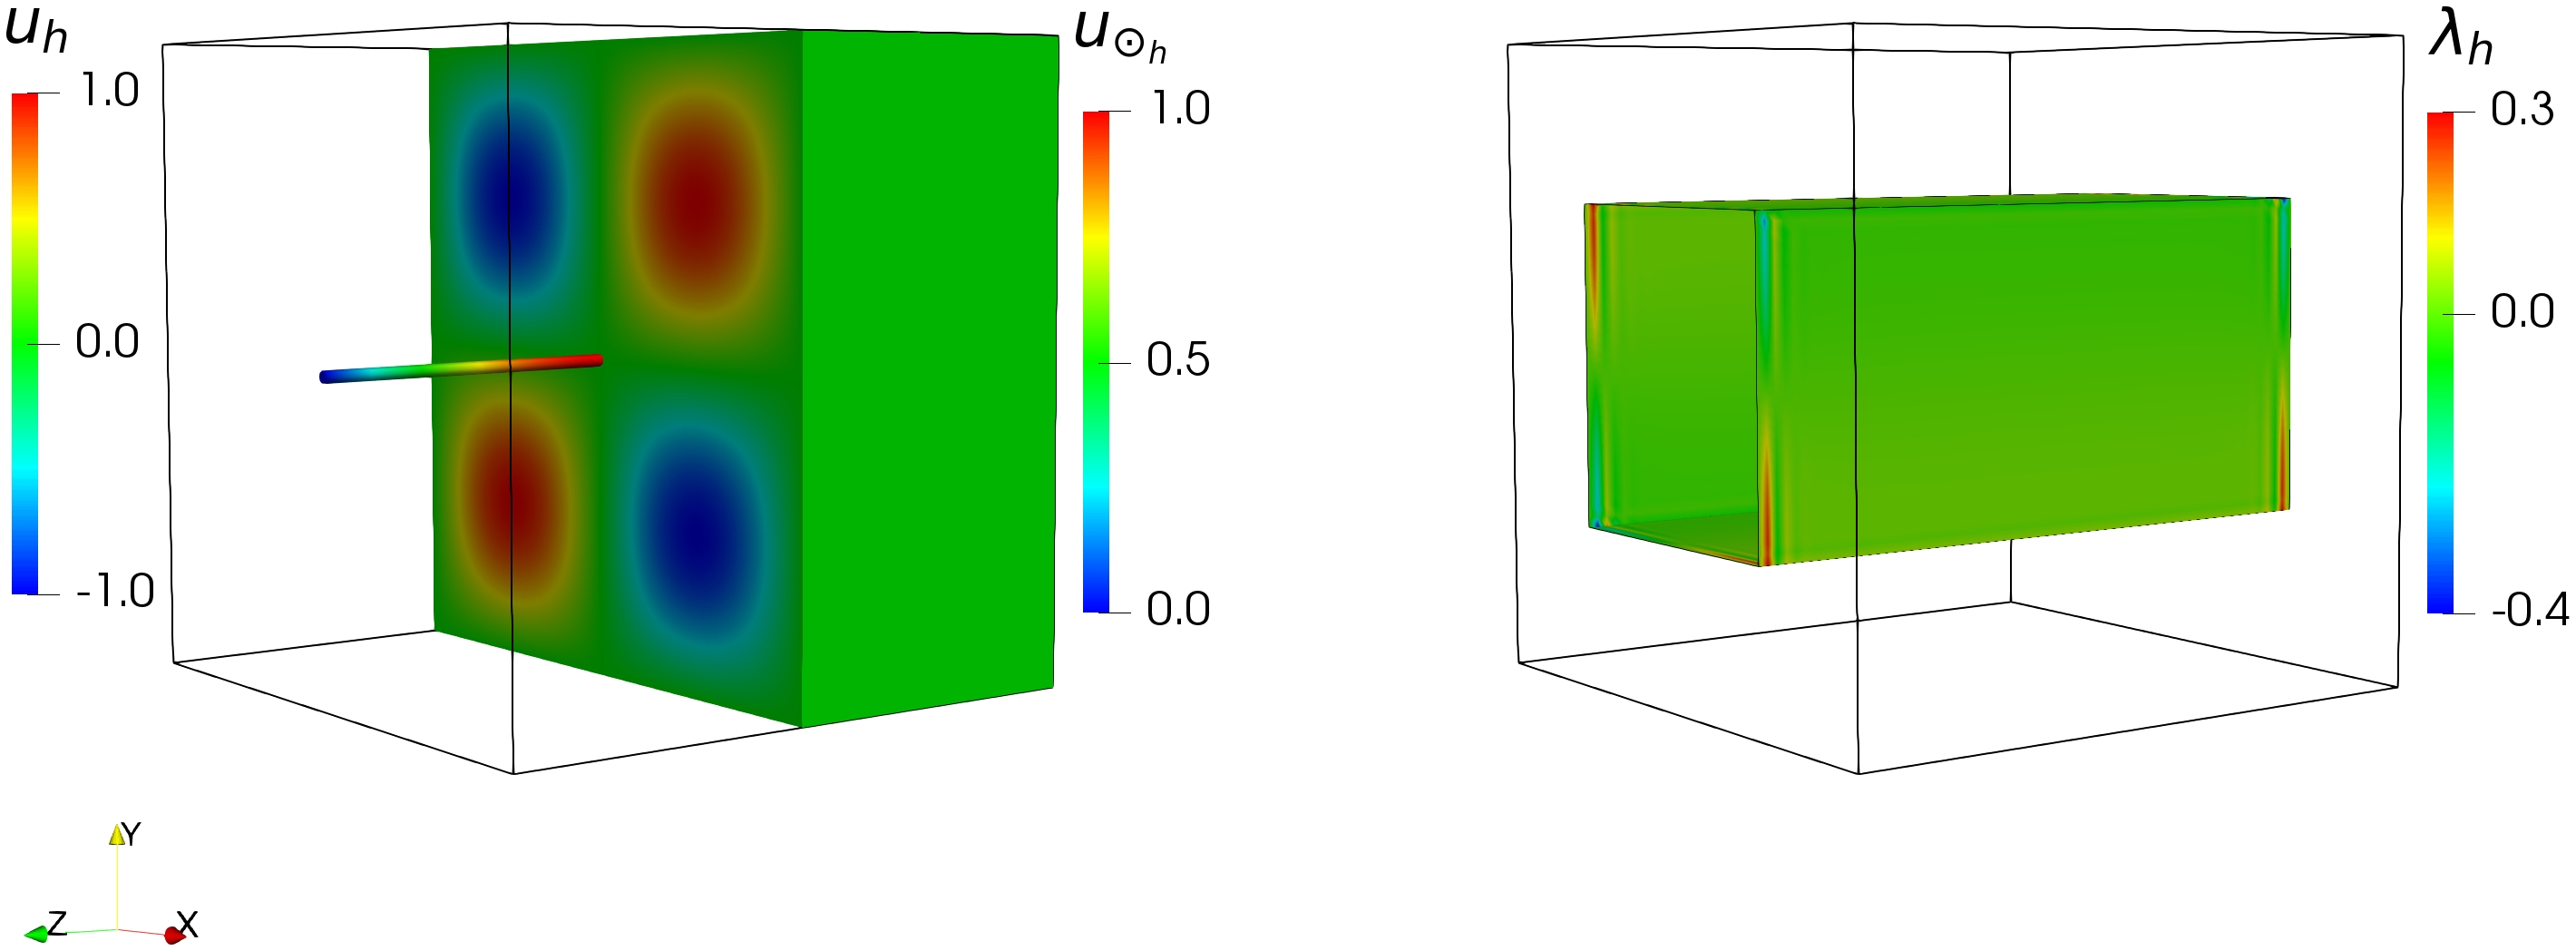
\includegraphics[width = 0.6\textwidth]{./graphics/mfs_LM2d}
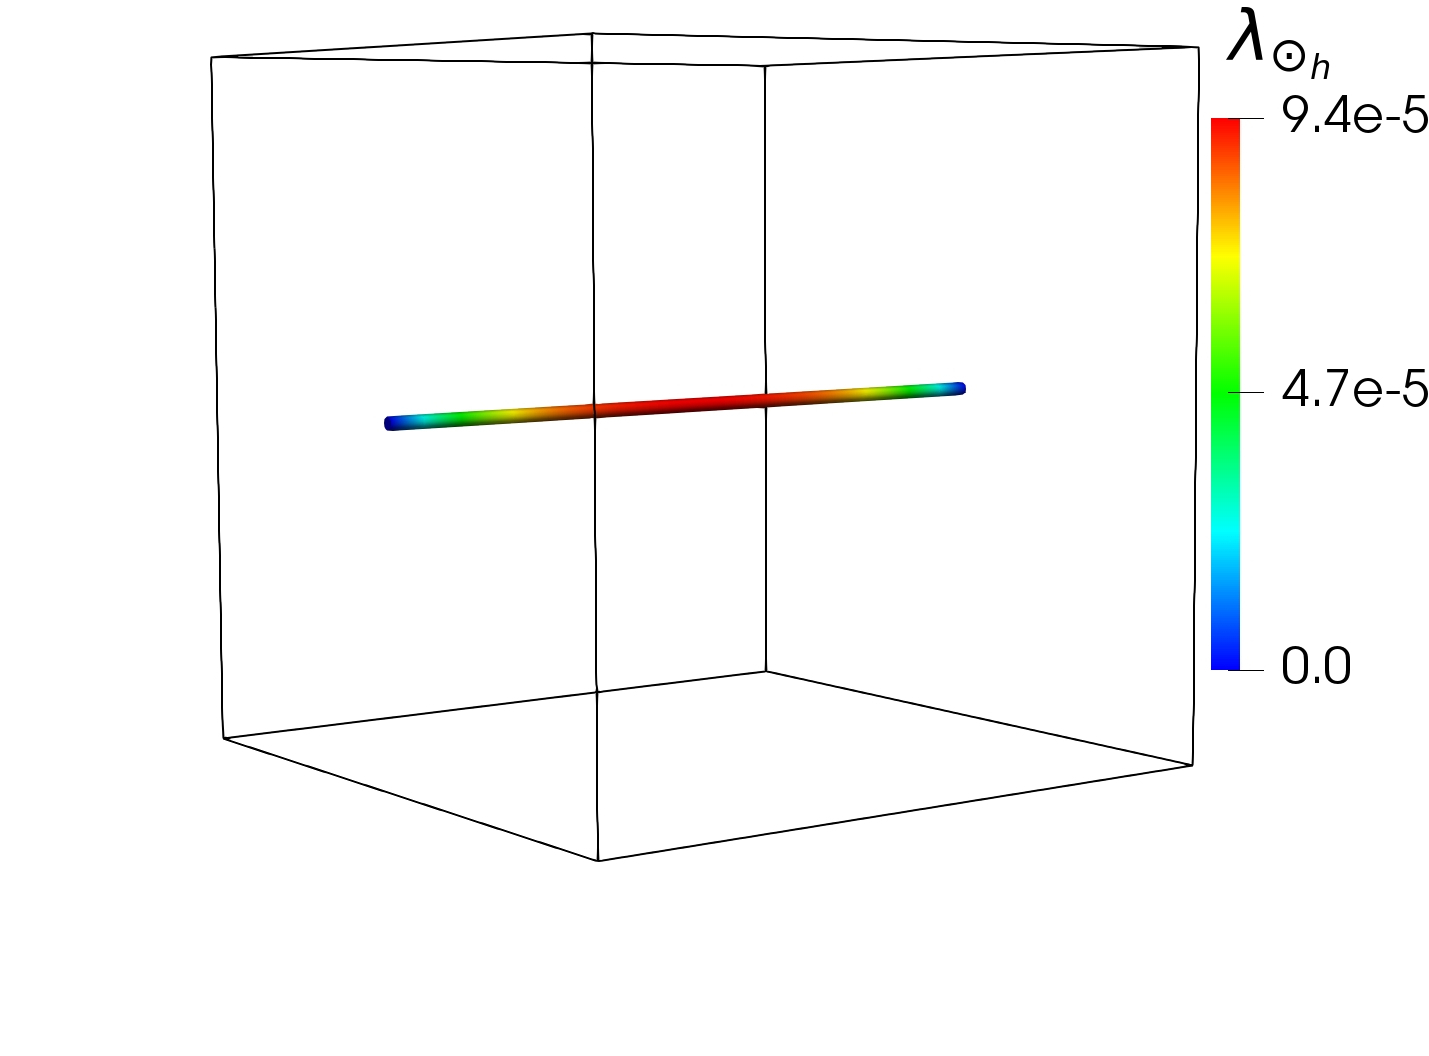
\includegraphics[width = 0.3\textwidth]{./graphics/mfs_LM1d_crop}
\vspace{-10pt}
\caption{Numerical solution of problem \eqref{eq:problem1} and
  \eqref{eq:problem2}. (Left) functions $u_h$, $\udh$ (practically identical
  in both problems). (Middle) Lagrange multiplier for \eqref{eq:problem1}
  and (right) for \eqref{eq:problem2}.}
\label{fig:sol_benchm1}
\end{figure}


%\begin{figure}
%\centering
%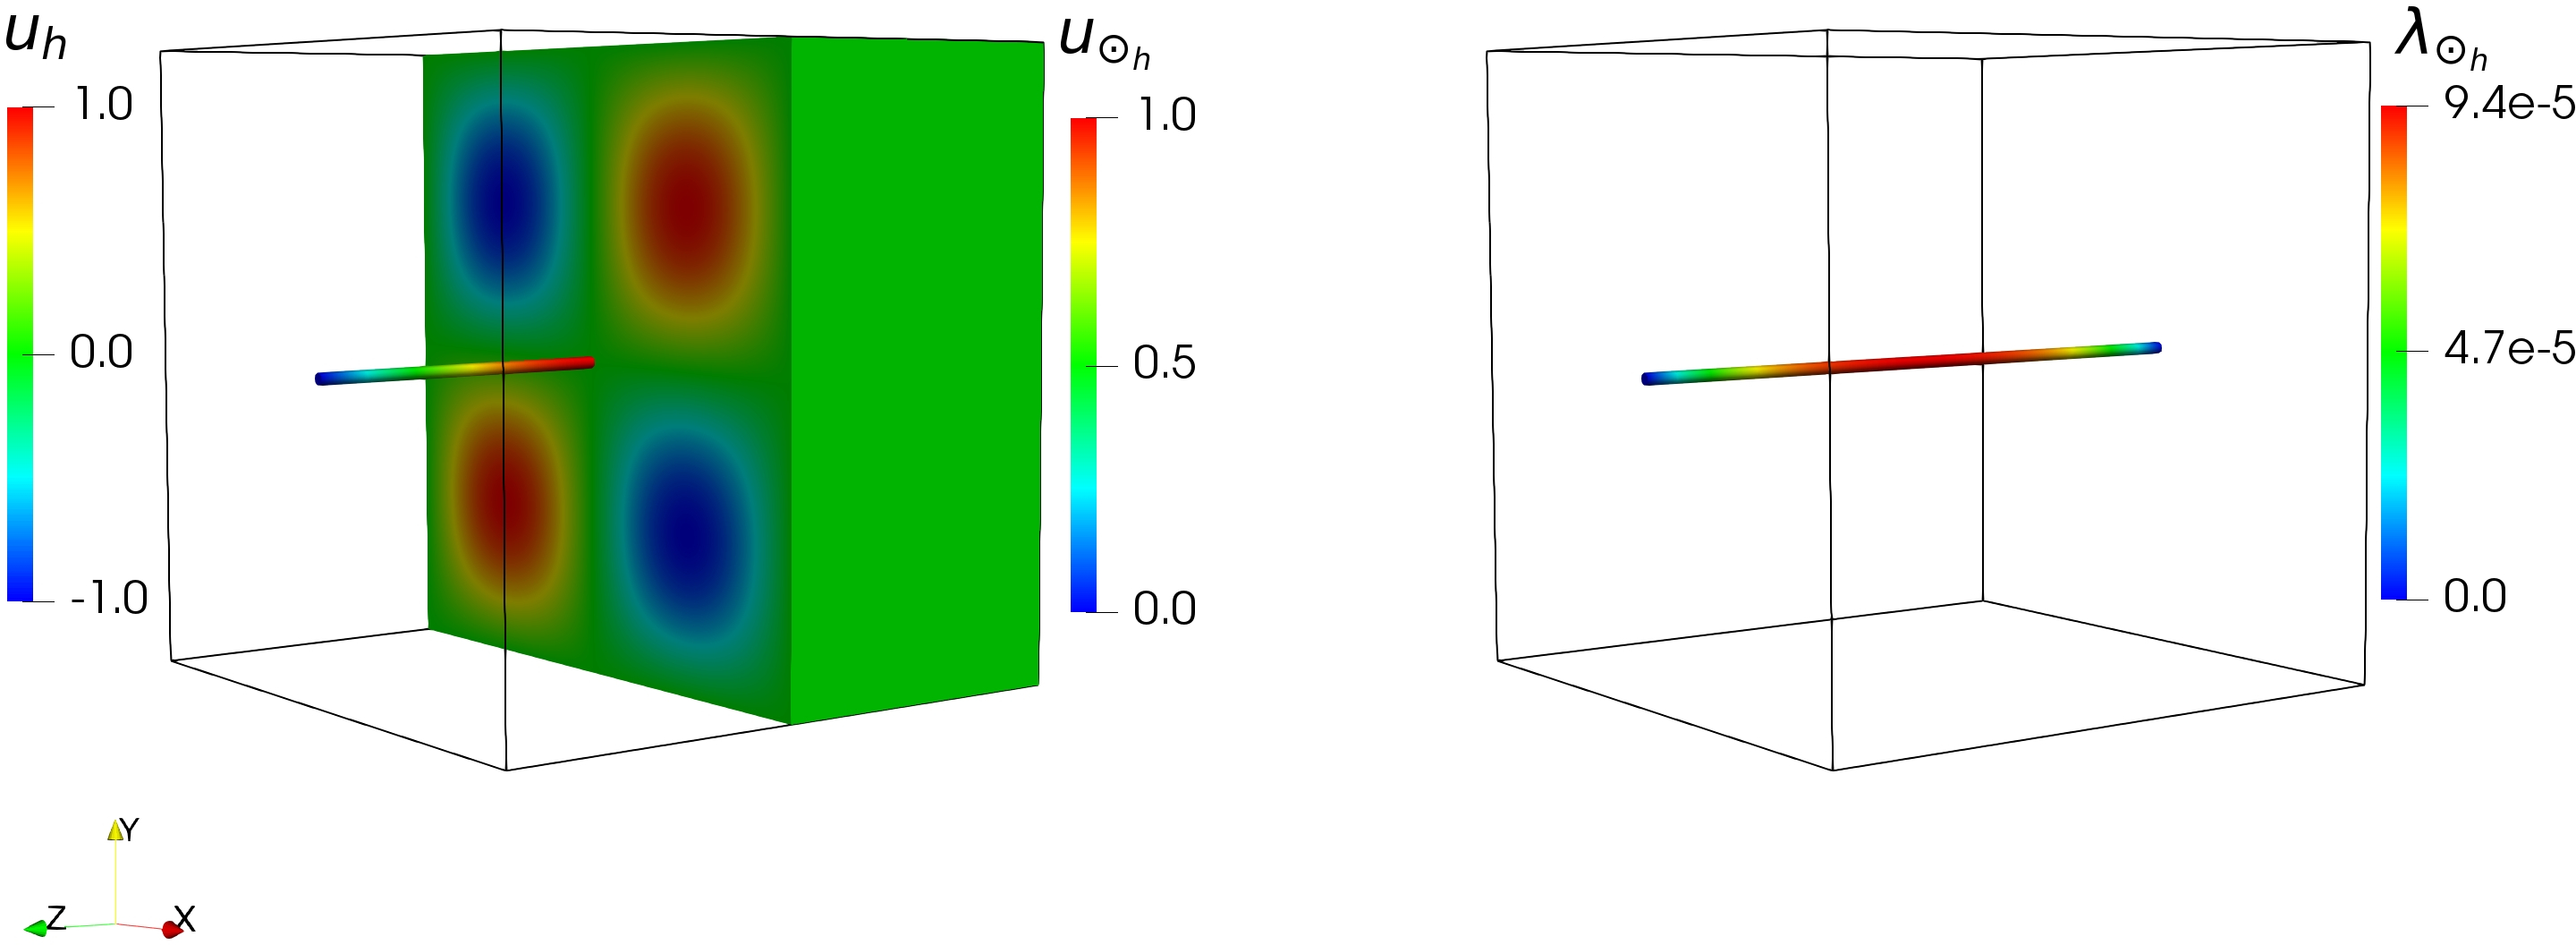
\includegraphics[width = 0.9\textwidth]{./graphics/mfs_LM1d}
%\caption{Numerical solution of problem \eqref{eq:problem2_simple}:
%  functions $u_h$ and $\udh$ on the left and the Lagrance multiplier
%  $\ldh$ on the right.}\label{fig:sol_benchm2}
%\end{figure}


\subsection{Numerical experiments. $\mathcal{T}^{\Omega}_h$ non-conforming to $\Gamma$}\label{sec:experiment_nonconform}
Using benchmark problem \eqref{benchmark} we consider \eqref{eq:problem2} in the
setting of \S \ref{sec:unfit2}. To this end we let $\mathcal{T}^{\Omega}_h$ be a uniform
mesh of $\Omega$ such that no cell $\mathcal{T}^{\Omega}_h$ has any edge
lying on $\Lambda$. Further we let $\mathfrak{h}=h/3$ in $\mathcal{T}^{\Lambda}_{\mathfrak{h}}$,
cf. Figure \ref{fig:mesh}.

Using discretization in terms of $P_1$-$P_1$-$P_0$ element Table \ref{tab:error_conform}
lists the error of the stabilized formulation of \eqref{eq:problem2}. A linear
convergence in the $H^1$ norm can be observed in the error of $u$ and $\ud$. We
remark that the norms were computed as in \S\ref{sec:experiment_conform}. For simplicity
the convergence of the multiplier is measured in the $L^2$ norm rather then the $H^{-1/2}(\Gamma)$
norm used in the analysis. Then, convergence exceeding order 1.5 can be observed, however,
the rates are rather unstable.


%% \begin{table}
%% %%   %%%
%% \begin{minipage}[b]{0.35\linewidth}
%%  \centering
%%  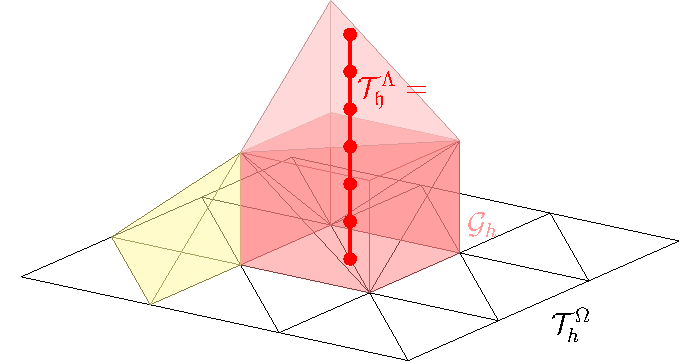
\includegraphics[width=\textwidth]{graphics/nonconform_mesh.pdf}
%%  \vspace{-20pt}
%%  \captionof{figure}{
%%    Sample discretization of the benchmark geometry in the non-conforming case. 
%%  }
%% \label{fig:unfit}
%% \end{minipage}
%% \hspace{2pt}
%% %%%
%%     \begin{minipage}[b]{0.62\linewidth}
%%       %%%
%%   \scriptsize{
%%   \begin{center}
%%     \begin{tabular}{l|lll}
%%       \toprule
%%     $h^{-1}$ & $\norm{u-u_h}_{1, \Omega}$ & $\norm{\ud-\udh}_{1, \Lambda}$ & $\norm{\ld-\ldh}_{0,\Lambda}$\\
%%       \hline
%% 5   & 2.6E0(--)    & 2.3E-1(--)   & 1.7E-1(--) \\ 
%% 9   & 1.5E0(0.84)  & 9.4E-2(1.42) & 7.1E-2(1.36)\\
%% 17  & 8.1E-1(0.94) & 4.3E-2(1.18) & 2.9E-2(1.37)\\
%% 33  & 4.2E-1(0.98) & 2.1E-2(1.06) & 7.9E-3(1.91)\\
%% 65  & 2.1E-1(0.99) & 1.1E-2(1.02) & 2.6E-3(1.64)\\
%% 129 & 1.1E-1(1.00) & 5.2E-3(1.01) & 8.5E-4(1.61)\\
%% \bottomrule
%%     \end{tabular}
%%   \end{center}    
%% }    
%%   \captionof{table}{
%%     Error convergence of \eqref{eq:problem2_simple} on a benchmark problem \eqref{benchmark} in case
%%     $\mathcal{T}^{\Omega}_h$ does not conform to $\Lambda$.}
%%   \label{tab:error_unfit}    
%%   \end{minipage}
%% \end{table}

\subsection{Comparison}
In Tables \ref{tab:error_conform} one can observe that 
all the formulations yield practically identically accurate approximations of $u$.
Further, compared to the conforming case, the stabilized formulation \eqref{eq:problem2}
results in a greater accuracy of $u_{\odot h}$ as the underlying mesh $\mathcal{T}^{\Lambda}_{h}$ is
here finer. Due to the different definitions in the three formulations, comparision of the Lagrange
multiplier convergence is not straightforward. We therefore limit ourselves to a
comment that in the $L^2$ norm all the formulations yield faster than linear convergence.
%
In order to discuss solution cost of the formulations we consider 
the resulting preconditioned linear systems. In particular, we shall compare
spectral condition numbers and the time to convergence of the preconditioned
minimal residual (MinRes) solver with the with stopping criterion requiring
the relative preconditioned residual norm to be less than $10^{-8}$. We remark
that we shall ignore the setup cost of the preconditioner.
%
Following operator preconditioning technique \cite{mardal2011preconditioning} we
propose as preconditioners for \eqref{eq:problem1} and \eqref{eq:problem2} in the
conforming case the (approximate) Riesz mapping with respect to the inner products of
the spaces in which the two formulations were proved to be well posed.
In particular, the preconditioner for the Lagrange multiplier relies on
(the inverse of) the fractional Laplacian $-\Delta^{-1/2}$ on $\Gamma$ for
\eqref{eq:problem1} and $\Lambda$ for \eqref{eq:problem2}.
A detailed analysis of the preconditioners will be presented in a separate
work. We remark that in both cases the fractional Laplacian was here realized
by spectral decomposition \cite{kuchta2016preconditioners}.
%
For the unfitted stabilized formulation \eqref{eq:problem2} the Lagrange multiplier preconditioner
uses a Riesz map with respect to the inner product due to $L^2(\mathcal{G}_h)$ and
the stabilization \eqref{eq:stab}, i.e.
\[
(\ldh, \mdh) \mapsto \sum _{K\in \mathcal{G}_h}\int_{K}\ldh \mdh + \sum _{K\in \mathcal{G}_h} \int_{\partial K \setminus \partial \mathcal{G}_h} h \llbracket \ldh \rrbracket \llbracket \mdh \rrbracket.
\]
This simple choice does not yield bounded
iterations. However, establishing a robust preconditioner in this case 
is beyond the scope of the paper and shall be pursued in the future works.
%
In Table \ref{tab:cost} we compare solution time, number of iterations and
condition numbers of the (linear systems due to the) three formulations.
Let us first note that the proposed preconditioners for \eqref{eq:problem1} and
\eqref{eq:problem2} in the conforming case seem robust with respect to discretization
parameter as the iteration counts and condition numbers are bounded in $h$.
We then see that the solution time for \eqref{eq:problem1} is about 2 times
longer compared to \eqref{eq:problem2} which is about 4 times more expensive
than the solution of the Poisson problem \eqref{benchm_3d}. This is in addition to the
higher setup costs of the preconditioner, which in our implementation involve solving
an eigenvalue problem for the fractional Laplacian. Therefore it is advantageous to keep
the multiplier space as small as possible. We remark that the missing
results for \eqref{eq:problem1} in Table \ref{tab:cost} are due to the
memory limitations encountered when solving the eigenvalue problem
for the Laplacian, which for finest mesh involves cca 32 thousand eigenvalues, cf. Appendix \ref{sec:appendix}.
%
Due to the missing proper preconditioner for the Lagrange multiplier block the
number of iterations in the third, unfitted formulation can be seen to approximately
double on refinement. 

\begin{table}
  \scriptsize{
  \begin{center}
    \begin{tabular}{l|lll|lll|lll|ll}
      %\toprule
      \hline
      \multirow{2}{*}{$l$} & \multicolumn{3}{c|}{\eqref{eq:problem1}} & \multicolumn{3}{c|}{\eqref{eq:problem2}} & \multicolumn{3}{c|}{ Stabilized \eqref{eq:problem2}} & \multicolumn{2}{c}{\eqref{benchm_3d}}\\
      \cline{2-12}
      & \# & $T\left[s\right]$ & $\kappa$ & \# & $T\left[s\right]$ & $\kappa$ & \# & $T\left[s\right]$ & $\kappa$ & \# & $T\left[s\right]$\\
      \hline
      1 & 20 & 0.03  & 15.56 & 9  & 0.02  & 3.04 & 21  & 0.01   & 9.70  &3 & $<0.01$\\ 
      2 & 35 & 0.06  & 16.28 & 17 & 0.03  & 4.67 & 31  & 0.03   & 15.87 &4 & $<0.01$\\ 
      3 & 38 & 0.14  & 16.64 & 22 & 0.06  & 6.25 & 53  & 0.15   & 32.93 &5 & 0.01   \\ 
      4 & 39 & 1.70  & 16.75 & 24 & 0.89  & 7.03 & 110 & 4.54   & 61.48 &5 & 0.12   \\ 
      5 & 38 & 12.04 & 16.78 & 20 & 5.21  & 5.02 & 232 & 59.43  & 94.25 &5 & 0.90  \\ 
      6 & -- & --    & --    & 17 & 28.77 & --   & 507 & 832.90 & --    &6 & 7.75  \\
      \hline
      %\bottomrule
    \end{tabular}
    \end{center}
    }
  \caption{Cost comparison of the formulations across refinement levels $l$.
    Number of Krylov  iterations (preconditioned conjugate gradient for \eqref{benchm_3d},
    MinRes otherwise) and the condition number of the preconditioned
    problem is denoted by $\#$ and $\kappa$ respectively. Time till convergence
    of the iterative solver (excluding the setup) is shown as $T$. 
  }
\label{tab:cost}
\end{table}



%{\color{red}
%\begin{remark} In the following some observations:\\
%
%\begin{itemize}
%\item \textbf{How do we compute the norm $\|\cdot \|_{H^{-\frac 12}}$ in Table \ref{tab:error_conform}?} The norm $\|\cdot \|_{H^{-\frac 12}}$ has been computed using a decomposition based on eigenvalues and eigenfuctions of $\Delta ^{-\frac 12}$.\\
%
%\item \textbf{Why $\lambda _h \neq \lambda$?} Since $\lambda = 0 \in Q_h$, we would expect $\lambda _h = \lambda$. However, first of all we suspect that for the approximation error an estimate similar to \cite[(11.26)]{steinbach2007numerical} holds, reported in the following
%\begin{equation*}
%\|u-u_h\|^2_{H^1} + \|\lambda - \lambda_h\|^2_{H^{-\frac 12}} \leq c_1 h^2|u|^2_{H^2} + c_2 h^3\|\lambda_h\|^2_{H^1_{pw}},
%\end{equation*}
%where $\|\cdot \|_{H^1_{pw}}$ is the broken $H^1$ norm. 
%So the error on the LM depends on the error on the solution. We suspect that if for example $u$ and $\ud$ are $P_2$ functions and we use a $P_2$ approximation (therefore $u = u_h$ and $\ud = \udh$), also $\lambda = \lambda_h$.\\
%
%\item \textbf{Why the error is larger close to edges, especially in Figure \ref{fig:sol_benchm1}?} 
%We suspect that the reasoning for why the error is larger close to edges and corner vertices is that the multiplier is
%related to $\nabla u \cdot \boldsymbol{n}$ and the normal in the corner or on the z-aligned edges in the figure is not well-defined. Btw, the oscillations are smaller if we impose Neumann
%bcs on z min and max surfaces of $\Omega$ (the rest has Dirichlet).
%\end{itemize}
%\end{remark}
%}


%>>>>>>>>>>>>>>>>>>>>>>>>>>>>>>>>>>>>>>>>>>>>>>>>>>
\bibliographystyle{siamplain}
\bibliography{3d1d}

\newpage

\appendix
\section{System sizes in benchmark formulations}\label{sec:appendix}
Below we list dimensions of the finite element spaces used to discretize
formualations \eqref{eq:problem1}, \eqref{eq:problem2} and stabilized
\eqref{eq:problem2} on different levels of refinement.

\begin{center}
  \scriptsize{
    \begin{tabular}{l|lll|lll|lll}
      \toprule
      \multirow{2}{*}{$l$} & \multicolumn{3}{c|}{\eqref{eq:problem1}} & \multicolumn{3}{c|}{\eqref{eq:problem2}} & \multicolumn{3}{c}{ Stabilized \eqref{eq:problem2}}\\
      \cline{2-10}
      & $\lvert X^1_{h, 0}(\Omega) \rvert$ & $\lvert X^1_{h, 0}(\Lambda) \rvert$ & $\lvert Q_h(\Gamma) \rvert$ &
      $\lvert X^1_{h, 0}(\Omega) \rvert$ & $\lvert X^1_{h, 0}(\Lambda) \rvert$ & $\lvert Q_h(\Lambda) \rvert$ &
      $\lvert X^1_{h, 0}(\Omega) \rvert$ & $\lvert X^1_{h^{\prime}, 0}(\Lambda) \rvert$ & $\lvert Q_h(\mathcal{G}_h) \rvert$\\
      \hline
     1& 125    & 5  & 40   & 125     & 5   & 5   & 180     & 13  & 24  \\
     2& 729    & 9  & 144  & 729     & 9   & 9   & 900     & 25  & 48  \\
     3& 4913   & 17 & 544  & 4913    & 17  & 17  & 5508    & 49  & 96  \\
     4& 35937  & 33 & 2112 & 35937   & 33  & 33  & 38148   & 97  & 192 \\
     5& 274625 & 65 & 8320 & 274625  & 65  & 65  & 283140  & 193 & 384 \\
     6& --     & -- & -    & 2146689 & 129 & 129 & 2180100 & 385 & 768 \\
      \bottomrule
    \end{tabular}
    }
    \end{center}

\end{document}
